\documentclass[reprint,english,notitlepage]{revtex4-1}  % defines the basic parameters of the document

% if you want a single-column, remove reprint

% allows special characters (including æøå)
\usepackage[utf8]{inputenc}
\usepackage[english]{babel}

%% note that you may need to download some of these packages manually, it depends on your setup.
%% I recommend downloading TeXMaker, because it includes a large library of the most common packages.

\usepackage{physics,amssymb}  % mathematical symbols (physics imports amsmath)
\usepackage{graphicx}         % include graphics such as plots
\usepackage{xcolor}           % set colors
\usepackage{hyperref}         % automagic cross-referencing (this is GODLIKE)
\usepackage{tikz}             % draw figures manually
\usepackage{listings}         % display code
\usepackage{subfigure}        % imports a lot of cool and useful figure commands
\usepackage{cprotect}
\usepackage{float}


% defines the color of hyperref objects
% Blending two colors:  blue!80!black  =  80% blue and 20% black
\hypersetup{ % this is just my personal choice, feel free to change things
    colorlinks,
    linkcolor={red!50!black},
    citecolor={blue!50!black},
    urlcolor={blue!80!black}}
%
%% Defines the style of the programming listing
%% This is actually my personal template, go ahead and change stuff if you want
\lstnewenvironment{python}{
	\lstset{ %
		inputpath=,
		backgroundcolor=\color{white!88!black},
		basicstyle={\ttfamily\scriptsize},
		commentstyle=\color{magenta},
		language=Python,
		morekeywords={True,False},
		tabsize=4,
		stringstyle=\color{green!55!black},
		frame=single,
		keywordstyle=\color{blue},
		showstringspaces=false,
		columns=fullflexible,
		keepspaces=true}
}{}

\lstnewenvironment{cpp}{
	\lstset{ %
		inputpath=,
		backgroundcolor=\color{white!88!black},
		basicstyle={\ttfamily\scriptsize},
		commentstyle=\color{magenta},
		language=C++,
		morekeywords={True,False},
		tabsize=4,
		stringstyle=\color{green!55!black},
		frame=single,
		keywordstyle=\color{blue},
		showstringspaces=false,
		columns=fullflexible,
		keepspaces=true}
}{}

\lstset{literate=
  {á}{{\'a}}1 {é}{{\'e}}1 {í}{{\'i}}1 {ó}{{\'o}}1 {ú}{{\'u}}1
  {Á}{{\'A}}1 {É}{{\'E}}1 {Í}{{\'I}}1 {Ó}{{\'O}}1 {Ú}{{\'U}}1
  {à}{{\`a}}1 {è}{{\`e}}1 {ì}{{\`i}}1 {ò}{{\`o}}1 {ù}{{\`u}}1
  {À}{{\`A}}1 {È}{{\'E}}1 {Ì}{{\`I}}1 {Ò}{{\`O}}1 {Ù}{{\`U}}1
  {ä}{{\"a}}1 {ë}{{\"e}}1 {ï}{{\"i}}1 {ö}{{\"o}}1 {ü}{{\"u}}1
  {Ä}{{\"A}}1 {Ë}{{\"E}}1 {Ï}{{\"I}}1 {Ö}{{\"O}}1 {Ü}{{\"U}}1
  {â}{{\^a}}1 {ê}{{\^e}}1 {î}{{\^i}}1 {ô}{{\^o}}1 {û}{{\^u}}1
  {Â}{{\^A}}1 {Ê}{{\^E}}1 {Î}{{\^I}}1 {Ô}{{\^O}}1 {Û}{{\^U}}1
  {œ}{{\oe}}1 {Œ}{{\OE}}1 {æ}{{\ae}}1 {Æ}{{\AE}}1 {ß}{{\ss}}1
  {ű}{{\H{u}}}1 {Ű}{{\H{U}}}1 {ő}{{\H{o}}}1 {Ő}{{\H{O}}}1
  {ç}{{\c c}}1 {Ç}{{\c C}}1 {ø}{{\o}}1 {å}{{\r a}}1 {Å}{{\r A}}1
  {€}{{\euro}}1 {£}{{\pounds}}1 {«}{{\guillemotleft}}1
  {»}{{\guillemotright}}1 {ñ}{{\~n}}1 {Ñ}{{\~N}}1 {¿}{{?`}}1
}



\usepackage{thmtools}
\DeclareMathOperator{\nullspace}{Nul}
\DeclareMathOperator{\collspace}{Col}
\DeclareMathOperator{\rref}{Rref}
%%\DeclareMathOperator{\dim}{Dim}

 % "meq": must be equal
\newcommand{\meq}{\overset{!}{=}}
\newcommand\numberthis{\addtocounter{equation}{1}\tag{\theequation}}

\newcommand{\R}{\mathbb{R}}
\newcommand*\Heq{\ensuremath{\overset{\kern2pt L'H}{=}}}
\usepackage{bm}
\newcommand{\uveci}{{\bm{\hat{\textnormal{\bfseries\i}}}}}
\newcommand{\uvecj}{{\bm{\hat{\textnormal{\bfseries\j}}}}}
\DeclareRobustCommand{\uvec}[1]{{%
  \ifcsname uvec#1\endcsname
     \csname uvec#1\endcsname
   \else
    \bm{\hat{\mathbf{#1}}}%
   \fi
}}
\usepackage[binary-units=true]{siunitx}

\makeatletter
\newcommand*{\balancecolsandclearpage}{%
  \close@column@grid
  \cleardoublepage
  \twocolumngrid
}
\makeatother

\newcounter{subproject}
\renewcommand{\thesubproject}{\alph{subproject}}
\newenvironment{subproj}{
\begin{description}
	\item[\refstepcounter{subproject}(\thesubproject)]
}{\end{description}}


\begin{document}
\title{On the Monte Carlo simulation of the Ising model of a 2D lattice with two-state magnetic spins using the Metropolis algorithm}   % self-explanatory
\author{Eivind Støland, Anders P. Åsbø}               % self-explanatory
\date{\today}                             % self-explanatory
\noaffiliation                            % ignore this

\begin{abstract}
Abstract
\end{abstract}

\maketitle                                % creates the title, author, date


\tableofcontents

\section{Introduction} \label{sec:I}

The Ising model is a widely popular model for the simulation of phase transitions in magnetic systems. In this report we will look at a 2D lattice of two-state magnetic spins and simulate at various temperatures in both the region where we expect the system to be magnetized, and where we expect it to not be magnetized. To perform our simulations, we will create a C++ program that performs Monte Carlo simulations of the Ising model using the Metropolis algorithm. We will be using periodic boundary conditions for our 2D lattice.

Firstly we will test our implementation by simulating a \(2\times 2\) lattice and comparing the numeric mean energy, mean magnetization, mean magnitude of magnetization, specific heat capacity and magnetic susceptibility to analytically derived values.

We will then investigate the stability of our implementation, by simulating a \(20\times 20\) lattice for both phases of the magnetization. We will look at how many Monte Carlo cycles are necessary to achieve the most likely state of the system. Furthermore, we will look at the amount of accepted spin flips during simulation, as well as the probability distribution \(P(E)\) of the energies of the system.

Lastly, we will attempt to find the critical temperature at which the phase transition occurs. This will be done by simulating various temperatures in near the critical temperature for lattices of various sizes, and then using the specific heat capacities and magnetic susceptibilities to estimate the critical temperature of each lattice, which in turn are used to estimate the critical temperature in the thermodynamic limit of a 2D lattice with infinitely many spins.


\newpage

\section{Formalism} \label{sec:II}

\subsection{The Ising Model} \label{sec:II:a}

The Ising model is a mathematical model of ferromagnetic systems. It is based on a set of particles in a lattice with either spin up or down, and the energy that a particle has is dependent on other adjacent particles and on an external magnetic field if there is one. We will be working with this model in the canonical ensemble. The energy of a configuration of such a system is:

\begin{align*}
E &= -J \sum\limits_{<kl>}^N s_k s_l - B \sum\limits_k^N s_k \numberthis \label{eq:ising_general_total_energy} \, ,
\end{align*}

where $J$ is a parameter determining the strength of the interaction between adjacent particles, $B$ is a parameter determining the strength of the external magnetic field, and $N$ is the number of particles. The notation $<kl>$ in the first sum indicates that we should sum over all adjacent particles, and the values summed over, $s$, are the spins of particles, where the subscripts denote which particle it belongs to. The spins can be $s = \pm 1$, which we often denote with an arrow pointing upwards ($\uparrow$) for $s = +1$ and a downwards pointing arrow ($\downarrow$) for $s = -1$.

In order to further proceed we need a probability that governs the system. For this purpose, the Boltzmann distribution is used:

\begin{align*}
P_i (\beta) &= \frac{e^{-\beta E_i}}{Z} \numberthis \label{eq:boltzmann_dist} \, ,
\end{align*}

where $\beta = (k_B T)^{-1}$, $E_i$ the energy of a specific configuration of the system, $Z$ is the partition function, and the subscript $i$ denotes the configuration of the system. The parameter $\beta$ contains $k_B$ which is the Boltzmann constant, and $T$ is the temperature. The partition function is a normalization factor for the probability distribution, and is the sum of all the possible Boltzmann factors:

\begin{align*}
Z &= \sum\limits_i^M e^{-\beta E_i} \numberthis \label{eq:ising_partition_function} \, ,
\end{align*}  

where $M$ is the amount of microstates of the system. The magnetization of a given configuration is given by the sum of all the spins:

\begin{align*}
\mathcal{M}_i &= \sum\limits_j^N s_j \numberthis \label{eq:ising_magnetization}
\end{align*}

The mean of a general variable, $Q_i$, can be defined as:

\begin{align*}
\langle Q \rangle &= \sum\limits_i^M Q_i P_i(\beta) \numberthis \label{eq:mean}
\end{align*}

The variance of said variable can be defined as:

\begin{align*}
\text{Var}(Q) &= \langle Q^2 \rangle - \langle Q \rangle^2 \, , \numberthis \label{eq:variance} 
\end{align*}

which relates to the standard deviation $\sigma_Q$:

\begin{align*}
\sigma_q &= \sqrt{\text{Var}(Q)} \numberthis \label{eq:standard_deviation}
\end{align*}

The heat capacity at constant volume $C_V$ is related to the variance of the energy as follows:

\begin{align*}
C_V &= \frac{1}{k_B T^2} \text{Var}(E) = \frac{1}{k_B T^2} (\langle E^2 \rangle - \langle E \rangle^2) \, ,\numberthis \label{eq:heat_capacity}
\end{align*}

and the magnetic susceptibility $\chi$ is related to the variance of the magnetization:

\begin{align*}
\chi &= \frac{1}{k_B T} \text{Var}(\mathcal{M}) = \frac{1}{k_B T} ( \langle \mathcal{M}^2 \rangle - \langle \mathcal{M} \rangle^2) \numberthis \label{eq:magnetic_susceptibility}
\end{align*}

In the following section we look at a sample system.


\subsubsection{Periodic \( 2 \times 2 \) square lattice with no external field} \label{sec:II:A:i}

We look at a system where we have particles in a 2x2 square lattice. A configuration of the system can be visualized as follows: \newline

\begin{center}
\begin{tabular}{cc}
$\bullet$ & $\bullet$ \\
$\bullet$ & $\bullet$
\end{tabular}  , \newline
\end{center}

where we change the dots out for arrows to mark the spin of the particles. A sample configuration of the system can be visualized as follows: \newline

\begin{center}
\begin{tabular}{cc}
$\uparrow$ & $\downarrow$ \\
$\downarrow$ & $\uparrow$
\end{tabular}  . \newline
\end{center}


We can denote the spins of the system as $s_{ij}$, where the index $i$ corresponds to the row the particle is in and $j$ to the column. With periodic boundary conditions, the total energy of the system is then given by:

\begin{align*}
E &= -J ( 2s_{11}s_{12} + 2s_{11}s_{21} + 2s_{22}s_{21} + 2s_{22}s_{12}) \numberthis \label{eq:2x2_sq_lattice_en}
\end{align*}

As there are two possible states that the particles can be in, and there are four particles total, there are $2^4 = 16$ microstates. We are interested in the possible energies of this system, and they are listed in table \ref{table:2x2_sq_lattice_en_and_mag} along with the total magnetization, where we have used \eqref{eq:2x2_sq_lattice_en} and \eqref{eq:ising_magnetization} to calculate these values. Note that the values in this table are sorted by macrostate, as some of the microstates are effectively equal because of the symmetries of the system. There are a total of 6 configurations with two spins pointing upwards, but these do not all have the same energy, which means that the macrostate of the system cannot be uniquely determined by the amount of spins that point up (or down for that matter). If the two spins pointing upwards are adjacent the total energy is 0, and there are four such configurations. If the two spins are not adjacent the total energy is $8J$, and there are two such states. As there are then two macrostates (different energies) corresponding to two spins pointing up, we need a second identifier. The degeneracy of these macrostates differ, and so by listing both the degeneracy and the amount of spins pointing up we can uniquely determine all the macrostates of the system. This was used in the table.

\begin{table}[H]
\centering
\caption{This table contains the energies and total magnetization for all possible macrostates of the Ising model with a 2x2 square lattice of particles. The uniqueness of the macro state is determined by the amount of spins that are up (first column) and the degeneracy of said state (second column). Both are needed, as in the case with two spins pointing up there are four configurations with the two upwards pointing spins being adjacent, and two with them not being adjacent.} \label{table:2x2_sq_lattice_en_and_mag}
\begin{tabular}{|c|c|c|c|}
\hline
Spins up & Degeneracy & Energy & Magnetization \\
\hline
4 & 1 & -8J & 4 \\
3 & 4 & 0 & 2 \\
2 & 4 & 0 & 0 \\
2 & 2 & 8J & 0 \\
1 & 4 & 0 & -2 \\
0 & 1 & -8J & -4 \\
\hline
\end{tabular}
\end{table}


We can calculate the partition function of the system using \eqref{eq:ising_partition_function}:

\begin{align*}
Z &= \sum\limits_i^M e^{-\beta E_i} \\
&= 2 \bigg(e^{8J\beta} + e^{-8J\beta} \bigg) + 12 \\
&= 4\cosh(8J\beta) + 12
\end{align*}

The probability distribution of the system is thus:

\begin{align*}
P_i(\beta) &= \frac{e^{-\beta E_i}}{4\cosh (8J\beta) + 12}
\end{align*}

The expectation value for the energy can be found as follows:

\begin{align*}
\langle E \rangle &= \sum\limits_i^M E_i P_i(\beta) \\
 &= -8J \frac{2e^{8J\beta}}{4\cosh (8J\beta) + 12} + 8J \frac{2e^{-8J}}{4\cosh (8J\beta) + 12} \\
 &= -8J\frac{2(e^{8J\beta} - e^{-8J\beta})}{4\cosh (8J\beta) + 12} \\
 &= -8J\frac{\sinh(8J\beta) }{\cosh (8J\beta) + 3} \numberthis \label{eq:2x2_energy}
\end{align*}

It is simple to see that $\langle M \rangle = 0$, so a more interesting measure would be the expectation value of the absolute of the magnetization. The expectation value for the absolute value of the magnetization can be found similarly:

\begin{align*}
\langle |\mathcal{M}| \rangle &= \sum\limits_i^M |\mathcal{M}_i| P_i(\beta) \\
 &= \frac{2e^{8J\beta} + 4}{\cosh (8 J \beta) + 3} \numberthis \label{eq:2x2_abs_magnetization}
\end{align*}

In order to find the heat capacity it is first necessary to find the expectation value of squared energy:

\begin{align*}
\langle E^2 \rangle &= \sum\limits_i^M E_i^2 P_i(\beta) \\
&= 64J^2 \frac{\cosh(8J\beta)}{\cosh(8J\beta) + 3}
\end{align*}

This gives us the heat capacity by equation \eqref{eq:heat_capacity}:

\begin{align*}
C_V &= \frac{1}{k_B T^2} ( \langle E^2 \rangle - \langle E \rangle^2) \\
&= \frac{192J^2}{k_B T^2} \frac{\cosh(8J\beta)}{(\cosh(8J\beta) + 3)^2} \numberthis \label{eq:2x2_heat_capacity}
\end{align*}

Lastly we also want to find the magnetic susceptibility of the system. In order to do that we need to find:

\begin{align*}
\langle \mathcal{M}^2 \rangle &= \sum\limits_i \mathcal{M}_i^2 P_i(\beta) \\
&= 8 \frac{e^{8J\beta} + 1}{\cosh(8J\beta) + 3}
\end{align*}

This gives us the susceptibility by using equation \eqref{eq:magnetic_susceptibility}:

\begin{align*}
\chi &= \frac{1}{k_B T} ( \langle \mathcal{M}^2 \rangle - \langle \mathcal{M} \rangle^2 ) \\
&= \frac{8}{k_B T} \frac{e^{8J \beta} + 1}{\cosh( 8J \beta) + 3} \numberthis \label{eq:2x2_susceptibility}
\end{align*}

All of these values we have calculated here can be compared with numerical results later on in order to evaluate the veracity of the numerical results.


\subsubsection{Periodic square lattice with no external field in the thermodynamical limit} \label{sec:II:A:ii}

Solving the two-dimensional Ising model is a highly non-trivial task, and so we will only list the resulting expressions in the case where there is no external field. These expressions were found by Lars Onsager so we refer to his work \citep{L.Onsager1944} instead of performing the calculations ourselves. The partition function is given by the following:

\begin{align*}
Z_N &= [2\cosh(\beta J) e^I ]^N \, , \numberthis \label{eq:LO_partition_function}
\end{align*}

where: 

\begin{align*}
I &= \frac{1}{2\pi} \int_0^\pi d\phi \, \ln \bigg[\frac{1}{2}\bigg( 1 + ( 1 - \kappa^2 \sin^2 \phi)^{1/2} \bigg) \bigg] \, , 
\end{align*}

and:

\begin{align*}
\kappa &= \frac{2\sinh ( 2\beta J) }{\cosh^2(2\beta J)} \, ,
\end{align*}

and $N$ is the number of particles. This determines the mean energy:

\begin{align*}
\langle E \rangle &= -J \coth( 2\beta J) \bigg[ 1 + \frac{2}{\pi} (2\tanh^2 (2\beta J) - 1) K_1(\kappa) \bigg] \, , \numberthis \label{eq:LO_energy}
\end{align*}

where:

\begin{align*}
K_1 (\kappa) &= \int_0^{\pi/2} \frac{d\phi}{\sqrt{1 - \kappa^2 \sin^2 \phi}} \, .
\end{align*}

The heat capacity is derived from this quantity again, and is found to be:

\begin{align*}
C_V &= \frac{4k_B}{\pi} (\beta J \coth(2\beta J))^2 \bigg( K_1(\kappa) - K_2(\kappa) \\ 
& \quad - (1 - \tanh^2 (2\beta J) ) \bigg[ \frac{\pi}{2} + (2\tanh^2 (2\beta J) - 1)K_1(\kappa) \bigg] \bigg) \, , \numberthis \label{eq:LO_heat_capacity}
\end{align*}

where:

\begin{align*}
K_2(\kappa) &= \int_0^{\pi/2} d\phi \, \sqrt{1 - \kappa^2 \sin^2 \phi}
\end{align*}

The mean magnetization per spin is given by:

\begin{align*}
\langle \mathcal{M} / N \rangle &= \bigg[1 - \frac{(1- \tanh^2 (\beta J) )^4}{16\tanh^4 (\beta J)} \bigg]^{1/8} \, , \numberthis \label{eq:LO_magnetization_per_spin}
\end{align*}

when the temperature is lower than a specific critical value $T_C$. Above this value the mean magnetization per spin is zero.

These solutions have the interesting feature that they predict a phase transition at this critical temperature $T_C$. The heat capacity, magnetization and susceptibility all excibit a power law behaviour (\citep{Stanley1999}, \cite[chapter 2.1.2]{landau_binder_2014}) in the region where $T\to T_C$ and $T$ is close to $T_C$. Specifically the heat capacity behaves as:

\begin{align*}
C_V &\sim \bigg| T_C - T \bigg| ^{-\alpha} \, , \numberthis \label{eq:power_law_heat_capacity}
\end{align*} 

when $T\to T_C$ from below, and $T$ is close to $T_C$. It can be determined that the correct solution is $\alpha = 0$, meaning that this behaves according to the power law singularity in the thermodynamic limit. The magnetization per spin behaves as:

\begin{align*}
\langle \mathcal{M} / N \rangle &\sim (T_C - T)^{\beta} \, , \numberthis \label{eq:power_law_magnetization_per_spin}
\end{align*}

in the same region, and with $\beta \to 1/8$. Similarly the susceptibility can be shown to behave as:

\begin{align*}
\chi &\sim |T_C - T|^{-\gamma} \, , \numberthis \label{eq:power_law_susceptibility}
\end{align*}

in the same region, and with $\gamma \to 7/4$. The correlation function, $C(r)$, where the parameter $r$ defines the distance between spins, is a measure of how much the spins correlate with each other, and can be shown \citep{Stanley1999} to scale as:

\begin{align*}
C(r) &\sim  e^{-r/\xi} \, ,
\end{align*}

where $\xi$ is the correlation length. As we approach the critical temperature we expect this to decay slower, as a change in a spin should quickly correlate to a change in another spin elsewhere. As $r$ is only dependent on how far apart the spins are the only variable that can cause this to happen is the correlation length, meaning that it has to get large as we approach the critical temperature. Because of this it can be shown that close to the critical temperature the correlation length also exhibits power law behaviour  (this is shown in \citep{Stanley1999}, albeit by a different route than the one outlined here):

\begin{align*}
\xi (T) &\sim |T-T_C|^{-\nu} \, , \numberthis \label{eq:power_law_correlation_length_} 
\end{align*}

where $\nu$ is a constant. A phase transition such as the one that the Ising model predicts is characterized by a correlation length that spans the whole system, and thus this correlation length can also be connected to the size of the system if we are looking at a finite lattice:

\begin{align*}
\xi (T) &\propto L \, ,
\end{align*}

where $L$ is the amount of spins in one direction in this finite lattice. Connecting this with the previous result we can define a connection between the critical temperature in a finite lattice and the one in the thermodynamical limit:

\begin{align*}
T_C(L) - T_C(L= \infty) &= aL^{-1/\nu} \, , \numberthis \label{eq:crit_temperature_finite_lattice} 
\end{align*}

where $a$ is a constant, and $\nu$ is the same constant as earlier. Combining this with the results for the heat capacity, the mean magnetization, and the magnetic susceptibility gives us the following relations in a finite lattice (\citep[p.78]{landau_binder_2014}):

\begin{align*}
C_V &\sim |T_C - T |^{-\alpha} \propto  L^{\alpha/\nu} \, , \numberthis \label{eq:finite_lattice_heat_capacity} \\
\langle \mathcal M \rangle &\sim (T-T_C)^\beta \propto L^{-\beta /\nu} \, , \numberthis \label{eq:finite_lattice_magnetization_per_spin} \\
\chi &\sim |T_C - T|^{-\gamma} \propto L^{\gamma/\nu} \, , \numberthis \label{eq:finite_lattice_susceptibility}
\end{align*}

where all variables are as defined earlier. We can use these relations to generate an estimate of $T_C(L)$, and if this is done for multiple $L$ we can estimate $T_C(L=\infty)$ by using equation \eqref{eq:crit_temperature_finite_lattice}. This allows us to calculate values for finite lattices numerically and relate them with results from the thermodynamic limit, which is essential as simulating an infinite is simply not possible. The analytical critical temperature with $\nu=1$ is (\citep{L.Onsager1944}):

\begin{align*}
\tilde{T}_C &= \frac{k_B T_C}{J} = \frac{2}{\ln(1 + \sqrt{2})} \approx 2.26919 \, , \numberthis \label{eq:crit_temperature_analytical}
\end{align*}

where we have scaled the temperature $\tilde{T}_C$ using $k_B$ and $J$ so that it is a dimensionless quantity.


\subsection{The Ising model and the Metropolis algorithm} \label{sec:II:b}

One method of simulating a system in the Ising model is through a Markov Chain Monte Carlo setup, where we iterate and flip spins depending on the change in total energy that flipping said spins incur. The Metropolis algorithm \citep{Metropolis} is one such setup which we will explain in this section.

We propose a change in a set of spins will cause a change in the total configuration of the system. Changing the configuration of the system from one (denoted $a$) to another (denoted $b$) incurs a change in the total energy defined by $\Delta E = E_b - E_a$. If the change in energy is negative we instantly accept the new configuration, as the second law of thermodynamics states that the system should always move towards equillibrium (lowest energy) in a closed system. If however the change is positive (meaning that the system, we wish to let probabilities determine whether or not we accept the new configuration. We can calculate the probability of moving from configuration $a$ to $b$ by using the Boltzmann distribution \ref{eq:boltzmann_dist} ($P_i(T)$ where $i$ denotes the configuration of the system):

\begin{align*}
P_{a\to b}(T)  &= \frac{P_b (T) }{P_a (T)} = e^{-\beta \Delta E }\, . 
\end{align*}

In this case we assume that the change in energy is positive number, so this is always smaller than one as we wish for a probability. We then draw a random number $r$ between $0$ and $1$ using a random number generator, and compare this to the probability of the transition $P_{a\to b}(T)$. If $r\leq P_{a\to b} (T)$ we accept the new configuration, otherwise we keep the previous configuration. The process up to this point can be called a Monte Carlo cycle. The Monte Carlo cycle is performed a sufficient amount of times until the system has stabilized, which is characterized by the macroscopic variables of the system being stable.

As we can see we need to somehow calculate $P_{a\to b} (T)$ in every Monte Carlo cycle, and as this contains an exponential this is computationally expensive. We can, however, modify the Monte Carlo cycle in such a way that there only are set values of $\Delta E$, which means that we can precalculate $P_{a\to b} (T)$. Doing this will cause a massive speed up in the calculation. We have not yet outlined how we propose a new configuration, and this will also be covered by this same method.

If we flip only one spin at a time, there are only five possible changes in energy $\Delta E$. The difference in energy between the states of a two dimensional lattice when one spin is flipped can be calculated using \eqref{eq:ising_general_total_energy}. Assuming no outside magnetic field gives us the difference between states \(1\) and \(2\) as:

\begin{align*}
	\Delta E = E_{2} - E_{1} = \left(-J \sum\limits_{<kl>}^N s_k^{2} s_l^{2}\right) -
	\left(-J \sum\limits_{<kl>}^N s_k^{1} s_l^{1}\right),
\end{align*}

where a superscript is used to denote which state the respective spins belong to.

Since we are only interested in the difference in energy from flipping a single spin in the lattice, we can assume that \(s_{k}^{1} = s_{k}^{2} = s_{k}\). Thus we can rewrite \(\Delta E\) as
\begin{align*}
 	\Delta E = J \sum_{<kl>}^{N} s_{k} \left(s_{l}^{1} - s_{l}^{2}\right).
\end{align*}

Furthermore, any spin can only be \(\pm 1\) and spin \(s_{l}\) is flipped such that \(s_{l}^{2} = -s_{l}^{1}\). From this it follows that \begin{align*}
	\left(s_{l}^{1} - s_{l}^{2}\right) = \left(s_{l}^{1} + s_{l}^{1}\right) = 2s_{l}^{1}.
\end{align*}

The difference in energy can then be written as

\begin{align*}
 	\Delta E = 2Js_{l}^{1} \sum_{<k>}^{N} s_{k}, \numberthis \label{eq:delta_e}
\end{align*}

where we only sum over \(k\), since only one spin \(s_{l}\) is flipped.
For a two dimensional lattice, each spin only has four neighbours, thus we can write out the sum for any randomly chosen \(s_{l}\) with neighbours \(s_{a}, s_{b}, s_{c}, s_{d}\) as

\begin{align*}
	\Delta E = 2Js_{l}^{1}\left(s_{a} + s_{b} + s_{c} + s_{d}\right) \numberthis \label{eq:singleflip_energy_change} \\
	\Delta E = 2J(\pm 1)\left[(\pm 1) + (\pm 1) + (\pm 1) + (\pm 1)\right]
\end{align*}

From this we see that if all spins \(s_{k}\) have the same sign we get
\begin{align*}
	\Delta E = \pm 2J(\pm 4) = \pm 8J.
\end{align*}
If three of the spins \(s_{k}\) have the same sign we get
\begin{align*}
	\Delta E = \pm 2J(\pm 2) = \pm 4J.
\end{align*}
If two of the spins \(s_{k}\) have the same sign we get
\begin{align*}
	\Delta E = \pm 2J(0) = 0.
\end{align*}
Thus we only have five possible diffrences in energy between states when we only flip one spin. We can also visualize the possible transitions as follows:

\begin{align*}
E = -4J \quad \begin{array}{ccc}
& \uparrow & \\
\uparrow & \uparrow & \uparrow \\
& \uparrow &
\end{array} \quad \to \quad E = 4J \quad \begin{array}{ccc}
& \uparrow & \\
\uparrow & \downarrow & \uparrow \\
& \uparrow &
\end{array} \, ,
\end{align*}

with $\Delta E = 8J$, 

\begin{align*}
E = -2J \quad \begin{array}{ccc}
& \uparrow & \\
\downarrow & \uparrow & \uparrow \\
& \uparrow &
\end{array} \quad \to \quad E = 2J \quad \begin{array}{ccc}
& \uparrow & \\
\downarrow & \downarrow & \uparrow \\
& \uparrow &
\end{array} \, ,
\end{align*}

with $\Delta E = 4J$,

\begin{align*}
E = 0 \quad \, \quad \begin{array}{ccc}
& \uparrow & \\
\downarrow & \uparrow & \uparrow \\
& \downarrow &
\end{array} \quad \to \quad E = 0 \,\,\,\, \quad \begin{array}{ccc}
& \uparrow & \\
\downarrow & \downarrow & \uparrow \\
& \downarrow &
\end{array} \, ,
\end{align*}

with $\Delta E = 0$, 

\begin{align*}
E = 2J \quad \begin{array}{ccc}
& \downarrow & \\
\downarrow & \uparrow & \uparrow \\
& \downarrow &
\end{array} \quad \to \quad E = -2J \quad \begin{array}{ccc}
& \downarrow & \\
\downarrow & \downarrow & \uparrow \\
& \downarrow &
\end{array} \, ,
\end{align*}

with $\Delta E = -4J$, and lastly:

\begin{align*}
E = 4J \quad \begin{array}{ccc}
& \downarrow & \\
\downarrow & \uparrow & \downarrow \\
& \downarrow &
\end{array} \quad \to \quad E = -4J \quad \begin{array}{ccc}
& \downarrow & \\
\downarrow & \downarrow & \downarrow \\
& \downarrow &
\end{array} \, ,
\end{align*}

with $\Delta E = -8J$. These are the only possible changes in energy. The other possible transitions are the ones above but in reverse, and the energy change is then just what is listed, but with the sign being flipped. 

With this in mind we can precalculate all the probabilities $P_{a \to b} (T)$ and use these. In the case where $\Delta E < 0$ we have that $P_{a\to b} (T) > 1$, which means that it seizes to be a proper probability, but if we draw a random number and compare it to this as outlined earlier, the test will always pass if $\Delta E < 0$, meaning that we do not have to handle this as a special case.

A problem we encounter at this point is how we model the periodic boundary conditions. If we use a square lattice, we can use the amount of spins in a dimension $L$ and the modulo operator to define a function $f(i,k)$ that takes a valid index $i$ and what is to be added to it $k$, and returns the correct index on the other side of the lattice if it is out of bounds:

\begin{align*}
f(i) &= (i+k+L)\%L \, , \numberthis \label{eq:periodic}
\end{align*}

where \% is the modulo operator in this case. Note that we add $L$ to the total as well, as the function could return a negative value if $k$ was negative otherwise. The function might still return a negative value, but we have assumed here that $|k|$ is never larger than $L$. 
 
We have established that flipping one spin at a time is beneficial to the speed of the calculation. For larger systems this is a very small change, and so it is a good idea to flip more than one spin in each Monte Carlo cycle. Also if we want a more random process each cycle, we can also pick random spins that we attempt to flip, which we also choose to do later on. Exactly how all this is performed is outlined in section \hyperref[sec:III]{III}.

Every time a spin is flipped we need to update total energy and magnetization. The change in energy is $\Delta E$ and this can simply be added to the total. The difference in magnetization can be found using \eqref{eq:ising_magnetization}, and subtracting \(M_{2} - M_{1}\) (subscript one denotes the magnetization before the spin is flipped, and 2 the magnetization after): 

\begin{align*}
	\mathcal{M}_2 - \mathcal{M}_{1} &= \sum\limits_j^N s_j^{2} - \sum\limits_j^N s_j^{1} =
	\sum\limits_{j}^{N}\left(s_{j}^{2} - s_{j}^{1}\right).
\end{align*}

Because we assume only spin \(s_{l}\) is flipped when changing states, the difference in magnetization becomes:

\begin{align*}
 	\mathcal{M}_2 - \mathcal{M}_{1} = \left(s_{l}^{2} - s_{l}^{1}\right).
\end{align*} 

Using that \(s_{l}^{1} = - s_{l}^{2}\), we get:

\begin{align*}
	\mathcal{M}_2 - \mathcal{M}_{1} = \left(s_{l}^{2} + s_{l}^{2}\right) = 2s_{l}^{2},
\end{align*}

which gives that:

\begin{align*}
	\mathcal{M}_2 = \mathcal{M}_1 + 2s_{l}^{2} \numberthis \label{eq:delta_m}
\end{align*}


\newpage

\section{Method} \label{sec:III}

In this report we present simulations of the Ising model, in two dimensions with periodic boundary conditions and no external field, using the Metropolis algorithm. We have chosen to implement our solver as a class in C++ called \verb+IsingMetropolis+, with framework to operate said class using command line arguments in a main program in C++. Processing the results is done in Python, and all the simulations performed in this report is automated in Python as well. In this section we will discuss details on how key calculations are performed. In general we scale all equations used in these calculations such that $k_B = J = 1$. This makes it so that we do not need any natural constants at all, which simplifies the implementation significantly. The programs used are all linked to in appendix \hyperref[A]{A}.

\subsection{Details on calculations and key functions} \label{sec:III:a}

\subsubsection{Initialization of system} \label{sec:III:a:i}

Firstly, we will discuss how the system is initialized. We implemented two ways of initializing the spin matrix, total energy and magnetization. They are generated as follows:

\begin{cpp}
// Initiate spin matrix and magnetization
if (randspin) {
  for (int x = 0; x < n_spins; x++) {
    for (int y = 0; y < n_spins; y++) {
      spin_matrix(x,y) = (RNG(gen) >= 0.5) ? -1 : 1;
      M += spin_matrix(x,y);
    }
  }
} else {
  spin_matrix.ones();
  M = n_spins2;
}


// Initial energy
for(int y =0; y < n_spins; y++) {
  for (int x= 0; x < n_spins; x++){
    E -=  double(spin_matrix(y,x)*
          (spin_matrix(periodic(y,n_spins,-1),x) +
          spin_matrix(y,periodic(x,n_spins,-1))));
  }
}
\end{cpp}

Depending on the boolean variable \verb+randspin+ the spin-matrix is either generated as having all spins up (if \verb+randspin+ is false) or having a random spin configuration (if \verb+randspin+ is true). The spin matrix is an Armadillo \citep{Armadillo} integer matrix, which lets us use the \verb+ones()+ function to set all the spins to one. In this case the magnetization is simply the same as the total amount of spins which is stores in the variable \verb+n_spins2+. The random configuration is generated by using a double for loop, and random values drawn from the standard library function \verb+rand()+. In this case, every spin value is added to the variable that stores the magnetization (\verb+M+) in the same double for loop. The energy cannot be calculated at the same time as the spin matrix is being generated, as it needs all the neares neighbours to be generated already. Thus this calculation is separated into a secondary for loop, which is used in both cases. In general calculation of energy and magnetization is based on equations  \eqref{eq:ising_general_total_energy} and \eqref{eq:ising_magnetization} respectively.


\subsubsection{Performing a Monte Carlo sweep} \label{sec:III:a:ii}

The following code snippet performs one Monte Carlo sweep (flipping several spins, one at a time) based on the Metropolis algorithm on the system:

\begin{cpp}
std::random_device rd;
std::mt19937_64 gen(rd());
std::uniform_real_distribution<double> RNG(0.0, 1.0);
// Loop over all spins
for(int y =0; y < n_spins; y++) {
  for (int x= 0; x < n_spins; x++){

    // Get random indices
    int ix = int(RNG(gen)*(double)n_spins);
    int iy = int(RNG(gen)*(double)n_spins);

    // Calculate change in energy
    int deltaE =  2*spin_matrix(iy,ix)*
                  (spin_matrix(iy,periodic(ix,n_spins,-1))+
                  spin_matrix(periodic(iy,n_spins,-1),ix) +
                  spin_matrix(iy,periodic(ix,n_spins,1)) +
                  spin_matrix(periodic(iy,n_spins,1),ix));


    // Flip spin if new config is accepted
    if ( RNG(gen) <= w(deltaE+8) ) {
      spin_matrix(iy,ix) *= -1;


      // Update energy and magnetization if spin is flipped
      M += double(2*spin_matrix(iy,ix));
      E += double(deltaE);

      // Count accepted configs
      accepted_configs++;
    }
  }
}
\end{cpp}

The amount of spins that we attempt to flip, according to the condition from the Metropolis algorithm (see section \hyperref[sec:II:b]{II.B}), in one sweep is equal to the amount of spins in the system. The obvious solution in this case is to iterate through all the spins and attempt to flip each one, but a better solution is to let which spins we attempt to flip be random. In a physical context it is more realistic that all spins might flip at any point in time, meaning that any kind of ordering to which spin might flip would be unrealistic. To model this we use the Mersenne Twister random number generator \citep{MersenneTwister} which is implemented in the C++ standard library to draw random indices each iteration in the double for loop. 

At this point the change in energy is calculated. In order to apply the periodic boundary conditions an inline function \verb+periodic()+ is used. This function is equivalent to equation \eqref{eq:periodic}. Related to this equation the arguments it takes as input is $i$, $L$, and $k$, in that order. Adding to an existing valid index using this function returns the corresponding index on the other side of the lattice if it would otherwise be out of bounds on another side of the lattice.

Following this a random number is drawn, and if the probability of the energy transition is larger than this number then the spin is flipped. The Armadillo \citep{Armadillo} vector \verb+w+ stores the probabilities of the transitions and is calculated as follows:

\begin{cpp}
arma::vec w = arma::zeros(17);
for (int de = -8; de<= 8; de+=4) {
  w(de+8) = exp(-de/temperature(i));
}
\end{cpp} 

As the energy change is always an integer (we scaled the equations so that $J=1$) we can shift it by the lowest allowed value and use it as an index. This lets us access the probabilities using the energy change directly, removing the need for any calculation of any indices of \verb+w+ during the Monte Carlo sweep. Note that there are more values in \verb+w+ than there are allowed configurations. This is because the energy change can only be multiples of $2$. Dividing by two every time would cause unnecessary mathematical operations, so we instead define \verb+w+ to have twice as many elements as there are possible transitions between configurations.

If the random number drawn is less then the probability of the transition of configuration, the condition passes and the spin is flipped. If this is done the energy change is added to the total energy, and the magnetization is updated as well. A counter that keeps track of how many transitions that are accepted is also incremented. For further details on the algorithm used in this section, see section \hyperref[sec:II:b]{II.B}. 


\subsubsection{Running simulations} \label{sec:III:a:iii}

Simulations are performed by running the \verb+run()+ method of the \verb+IsingMetropolis+ class. As the program can run a simulation for a single temperature, or several simulations with different temperatures (all with the same lattice dimensions), this method is simply a wrapper that calls the correct function to run the simulation(s). In the case where a simulation is run for a single temperature, the following code snippet is used to run the simulation:

\begin{cpp}
double E = 0;
double M = 0;
arma::Mat<int> spin_matrix(n_spins,n_spins,arma::fill::ones);
arma::vec w = arma::zeros(17);
for (int de = -8; de<= 8; de+=4) {
  w(de+8) = exp(-de/temp);
}

initialize(randspin,spin_matrix,E,M);

for (int current_cycle = 1; current_cycle<=max_cycles; 
	 current_cycle++){
  one_monte_carlo_cycle(spin_matrix,E,M,w);
  write_to_file_single(E,M);
}
\end{cpp}

This implementation is quite straight forward. Doubles are created to store the energy and magnetization of the system, the spin matrix is instantiated, and \verb+w+ is generated as outlined in the previous section. Following this the system is initialized using the \verb+initialize()+ method which was covered in section \hyperref[sec:III:a:i]{III.A.1}. Then we loop our the specified amount of Monte Carlo cycles (\verb+max_cycles+), calling the method \verb+one_monte_carlo_cycle()+ which is the code snippet covered in section \hyperref[sec:III:a:2]{III.A.2}. In the loop the method \verb+write_to_file_single()+ is called, which does exactly what you would expect: it writes the results of the simulation to a file. This method writes the energy and magnetization per spin, and the total number of accepted configurations for each Monte Carlo cycle. 

If a set of simulations with the same lattice dimensions and varying temperatures are to be performed, the following code snippet is used:

\begin{cpp}
// Setting up parallelization and timing of simulation
int max_threads = omp_get_max_threads()*3/4;
int thrds = std::min(max_threads, n_temps);
std::cout << "Simulating L = " << n_spins << " with " 
		  << thrds << " threads." << std::endl;
double wtime = omp_get_wtime ( );

// Parallelized for loop
#pragma omp parallel for num_threads(thrds)
for (int i = 0; i<n_temps; ++i) {
  // Define local variables so the different threads do not use 
  // the same variables.
  arma::vec average = arma::zeros(5);
  double E = 0;
  double M = 0;
  arma::Mat<int> spin_matrix(n_spins,n_spins,arma::fill::ones);
  arma::vec w = arma::zeros(17);
  for (int de = -8; de<= 8; de+=4) {
    w(de+8) = exp(-de/temperature(i));
  }

  // Initialize spin matrix
  initialize(randspin,spin_matrix,E,M);

  for (int current_cycle = 1; current_cycle<=max_cycles; 
  	   current_cycle++){
    one_monte_carlo_cycle(spin_matrix,E,M,w);
    average(0) += E;
    average(1) += E*E;
    average(2) += M;
    average(3) += M*M;
    average(4) += fabs(M);
  }
  // Only one core should call this function at a time
  #pragma omp critical
  write_to_file_multi(average, temperature(i));
}
wtime = omp_get_wtime ( ) - wtime;
std::cout << "Finished simulating L = " << n_spins << " with " 
	      << thrds << " threads."
  		  << "\nElapsed time in seconds = " << wtime << std::endl;
\end{cpp} 

A for loop is used to iterate over the temperatures, and a simulation is performed for each of them. As these simulations are completely independent from each other, parallelizing this code using OpenMP is fairly straight forward, and we have done so in order to increase the efficiency of the simulation. We only need to make sure that the variables that are independent to the simulation are not shared. 

In general this functions very similarly to the previous code snippet inside this parallelized for loop. There are some key differences however. The most important one (which also happens to be related to all the differences) is that we do not write results to file each Monte Carlo cycle, instead we write to file once after a simulation is completed. What we write to file this time is also different than previously, and as some calculations are performed inside the \verb+write_to_file_multi()+ method, we will cover this shortly after we have finished outlining what is happening in this code snippet. The \verb+write_to_file_multi()+ method is passed an Armadillo \citep{Armadillo} vector containing mean energy, energy squared, magnetization, magnetization squared and absolute of magnetization. Along with this vector the temperature at which the simulation was ran is passed as an argument. In order to make sure that several threads do not write to the output file at the same time (which might result in cluttered lines) this call is defined as a critical section using OpenMP.

Outside the loop of the temperatures, the double \verb+wtime+ is used to measure the amount of time it takes to run all the simulations. Before the simulations start the amount of threads allocated is printed to the terminal, and after they are finished the time spent is also printed to the terminal. We use this to benchmark the simulations, with respect to both the parallelization and to compiler flags.

After each of the simulations are finished, we write the mean energy, magnetization and absolute of magnetization to file. We also calculate the heat capacity and the magnetic susceptibility as well, using the mean energy squared and magnetization squared along with their non-squared counterparts:

\begin{cpp}
// Normalizing factor
double norm = 1/(double(max_cycles));

// Extract averages
double Eaverage = average(0)*norm;
double E2average = average(1)*norm;
double Maverage = average(2)*norm;
double M2average = average(3)*norm;
double Mabsaverage = average(4)*norm;

// Calculate heat capacity and susceptibility
double heat_capacity = (E2average- Eaverage*Eaverage)
					   /(n_spins2*temperature*temperature);
double susceptibility = (M2average - Mabsaverage*Mabsaverage)
					    /(n_spins2*temperature);

// All expectation values are per spin, divide by 1/(n_spins^2)
Eaverage /= n_spins2;
Maverage /= n_spins2;
Mabsaverage /= n_spins2;
\end{cpp}

The Armadillo \citep{Armadillo} vector \verb+average+ contains the values we need, so these are extracted and then used to calculate the heat capacity and susceptibility. We calculate the heat capacity and magnetic susceptibility using equations \eqref{eq:heat_capacity} and \eqref{eq:magnetic_susceptibility}, where we have scaled the equations such that $k_B = 1$. Note that the absolute of the magnetization is used to calculate the magnetic susceptibility instead of the magnetization itself, as the former is a much more stable measure of what is actually happening when the magnetization gets close to zero.

When the averages are extracted from the vector, note that we multiply by a normalizing factor. This is because when calculating the varlues that are stored in \verb+average+ we have only added to their total in each Monte Carlo cycle. To actually get the average we need to divide by the amount of cycles, which is what is done by multiplying with the normalizing factor. Also note that we are interested in values per spin, so we divide by the total amount of spins (stored in variable \verb+n_spins2+) in all of the values. As we do not write mean energy squared and magnetization squared to file, dividing them by the amount of spins as well would be redundant and is therefore not done.

Our system has a total of \(24\) threads available (see \hyperref[C]{appendix C}), and since the simulation of multiple temperature values is parallelized by running one simulation thread for each temperature, we end up leaving quite a few unused threads when we run the parallelized simulation for \(8\) temperatures. To take advantage of the remaining threads, we introduce another level of parallelization in the \verb+project.py+ python-script:
\begin{python}
def phase_trans_test(nmax, Ls, files, n_temps):
    """Function running simulations for phase transition.
    Runs the cpp program for each L-value. If enough threads are
    available, multiple instances of the cpp program are run
    concurrently.

    Arguments:
    nmax -- int: number of Monte Carlo cycles to perform.
    Ls -- iterable: iterable containing the L-values to simulate.
    files -- iterable: iterable containing the filenames to
    				   write data to.
    n_temps -- int: number of temperatures to simulate in interval
                    [Tmin, Tmax].
    """
    Tmin, Tmax = 2.2, 2.35  # min and max temp.

    # number of concurrent subprocesses to spawn
    n_thrds = np.max([mp.cpu_count()//n_temps, 1])

    def phase_L_sim(i):
        """Function spawning subprocess and returning it."""
        p = Popen(
            [
                "./main.exe",
                files[i],
                "multi",
                f"{Ls[i]}",
                f"{nmax}",
                f"{Tmin}",
                f"{Tmax}",
                f"{n_temps}"
            ],
            cwd=src
        )
        return p

    # sets number of subprocesses to spawn at the same time:
    ranges = [len(Ls[i:i+n_thrds])
    		  for i in range(0, len(Ls), n_thrds)]
    		  
    # iterating through number of subprocesses
    # to spawn at the same time:
    print("Spawning subprocesses:")
    sims = [phase_L_sim(j) for j in range(ranges[0])]

    # loop checking status of subprocesses,
    # and spawning new subprocesses when a current one finishes.
    i = len(sims)
    while i < len(Ls):
        for p in sims:
            if p.poll() is not None:
                print("Spawning subprocesses:")
                sims.append(phase_L_sim(i))
                i += 1

    # waiting for all subprocesses to finish
    [p.wait() for p in sims]
\end{python}
The above python function takes in a list of lattice dimensions \(L\), and spawns independent instances of the C++ program for each \(L\), such that the maximum amount of possible threads are used during simulation. In our case we have \(8\) threads for each value of \(L\), meaning we can simulate \(3\) values of \(L\) at any given time, resulting in \(3\cdot 8 = 24\) threads being used.

\subsubsection{Calculation and comparison of results} \label{sec:III:a:iv}

The C++ programs output results to a file. Depending on the kind of run that is performed (see section \hyperref[sec:III:b]{III.B} for more details on this) the programs will either write results once per Monte Carlo sweep or once at the end of a simulation. If a single simulation (for one temperature) is performed the programs write total energy and magnetization to file once per Monte Carlo sweep. This is used to evaluate how quickly the solutions stabilize. The programs also have the possibility to run simulations for several temperatures with one run, and in this case the mean energy, mean magnetization, mean absolute value of magnetization, heat capacity, magnetic susceptibility and temperature is written to file at the end of each simulation. In this case the heat capacity and magnetic susceptibility are calculated using equations \eqref{eq:heat_capacity} and \eqref{eq:magnetic_susceptibility} respectively.

In post-processing these results can be used to estimate the critical temperature of the system. From the relations listed in equations \eqref{eq:power_law_heat_capacity}, \eqref{eq:power_law_magnetization_per_spin} and \eqref{eq:power_law_susceptibility} we can estimate the critical temperature from the behaviour of heat capacity, magnetization and magnetic susceptibility as functions of the temperature. As the exponent in the expressions for the heat capacity and magnetic susceptibility are negative, we expect that these will diverge closer to the critical temperature. In a numerical simulation of a finite lattice they will never actually diverge, but we still expect them to reach maximum values around the critical temperature, and this gives us two estimates of the critical temperature. 

Using the magnetization, however, is a bit more tricky. As the exponent is positive, it is supposed to reach zero at the critical temperature. In a numerical simulation this will never happen, as when the temperature gets large enough it will oscillate around zero. In order to combat this slightly we can use the absolute value of the magnetization instead. In this case there will still be problems though, as it will never stabilize at zero. In fact, the smaller the lattice is, the more it will vary. With all this in mind it is difficult to estimate the critical temperature using the magnetization. Thus we omit using the magnetization in our estimation of the critical temperature.

We now have two estimates of the critical temperature. In order to obtain our final estimate we choose to average these two. This estimate is now an estimate of the critical temperature for a specific size of the lattice. These simulations can be repeated for other lattice sizes as well, and these estimates can then be used together along with equation \eqref{eq:crit_temperature_finite_lattice} in order to estimate the critical temperature in the thermodynamical limit. All of the calculations explained here are performed in the following Python function:

\begin{python}
def get_critical_temperature(Ls, Cv, Xi, T):
    """Function calculating critical temperature from phase
    transition data.

    Returns tuple where first element is critical temperature at
    the thermodynamical limit (float). Second element is array
    containing mean of critical temperatures for each value of L.

    Arguments:
    Ls -- iterable: iterable containing the simulated L-values.
    Cv -- iterable: iterable containing the values of the specific
    				heat.
    Xi -- iterable: iterable containing the values of the
    				susceptibility.
    T -- iterable: iterable containing the values of
    			   temperature.
    """
    TC = np.zeros(len(Ls))
    for i, L in enumerate(Ls):
        # Get data arrays
        Cvi = Cv[i, :].flatten()
        Xii = Xi[i, :].flatten()

        # Find critical temperature as maximum point of
        # heat capacity
        TcCv = T[np.where(Cvi == np.max(Cvi))]

        # Find critical temperature as maximum point in
        # susceptibility
        TcXii = T[np.where(Xii == np.max(Xii))]

        # Average the three values found for final value
        TC[i] = (TcCv + TcXii)*0.5

    # Fitting critical temperature as a function of L to estimate
    # critical temperature at L=inf
    p, V = np.polyfit(1/np.array(Ls), TC, 1, cov=True)
    return p[1], np.sqrt(V[1][1]), TC
\end{python} 

The variable \verb+Ls+ contains the dimensionality of the lattice for the various simulations, \verb+absM+ contains the mean absolute of the magnetization, \verb+Cv+ contains the heat capacity, \verb+Xi+ contains the magnetic susceptibility, and \verb+T+ contains the temperatures. 

We use NumPy \citep{numpy} functions throughout our implementation, as NumPy arrays are both practical and have useful built-in functions that can act upon these that significantly simplify the calculations we perform in Python. In this case we use them to identify the maximum points in the two arrays for heat capacity and magnetic susceptibility using \verb+numpy.where()+ function which returns the indices at which the argument are true (argument should be a boolean array). We also use the \verb+flatten()+ member function of arrays which reduces the array to a 1-dimensional array. This is to avoid any unwanted nesting that might show up. Lastly, \verb+numpy.polyfit()+ is used to fit the calculated critical temperatures at different lattice lengths $L$ to the first order polynomial given in \eqref{eq:crit_temperature_finite_lattice}. The constant term from this fit is our estimate of the critical temperature in the thermodynamic limit. NumPy's \verb+polyfit()+ function can also return the covariance matrix, of which the second diagonal element is the uncertainty in the constant term from the fit. The function returns all of the critical temperature estimates and the uncertainty in the critical temperature for an infinite lattice from the fit.


\subsection{Unit-testing} \label{sec:III:B}

We were only able to device one good unit-test for the system. As this is a Monte Carlo simulation, and is based on pseudo-random numbers it is impossible to find set ways in which test the outcomes of the parts of the program behave other than with using seeds. If we use a set seed, however, this causes the simulations to be deterministic, which in general is not a desirable outcome. The only way we can truly test these as a whole is to compare to analytical results, and of those we have two that we can compare with. We have the results for the 2$\times$2 lattice described in section \hyperref[sec:II.A.i]{II.A.1} and the infinite lattice results found by Lars Onsager \citep{L.Onsager1944} which we listed in section \hyperref[sec:II.A.ii]{II.A.2}. The latter one is not possible to simulate numerically, and in order to compare our results to these we would need to run several simulations for large lattice dimensions, and use the power series approximations listed in the same sections to relate the results to the ones from the infinite lattice. This is very time-consuming, and is thus not well suited as a unit-test. The results from the $2\times2$ lattice however can easily be compared to the numerical results with a minimal amount of simulation time. Thus we have written a unit-test in Python that runs this simulation and compares the results to the analytical ones.     


\subsection{Error sources} \label{sec:III:C}

We need to discuss the potential error sources in these simulations, so that we can establish our expectation of how they will manifest. As in all numerical simulations there is room for error here as well. Notably, however, machine precision and truncation errors will most likely not be playing a significant part in errors in the results, as we are hard-pressed to go beyond a few significant digits in any of the quantities calculated. Both the energy and magnetization are stored as doubles, but we only add or subtract integers to their values. This is prone to numerical error, but as long as we are not running for very large lattice dimensions (larger than $1000\times 1000$) the order of magnitude for the energy and magnetization will typically never be more than 6 orders of magnitude larger than the integers that are added to them. This should not cause any kind of sizeable truncation error. 

What can cause an error in this case however is adding the variables into the vector \verb+average+ (see section \hyperref[sec:III:A:iii]{III.A.3}). If the simulations are long enough (a large amount of Monte Carlo cycles) there is cause for worry that we might encounter a loss of precision when adding values to the vector \verb+average+, or even potentially an overflow or an underflow. The potential overflow or underflow can largely be ignored, as we elect to use doubles to store the variables which can hold extremely large numbers. The loss of precision, however, is something we need to quantify more accurately, as the difference in order of magnitude could get large. We need to find out how many Monte Carlo cycles are needed before we lose significant digits. 

If we assume all of the quantities that are added to the vector are of the same order of magnitude (this is not a bad approximation as they should stabilize around a given value), the order of magnitude of the double stored in the vector should be $\log_{10}(n)$ times the order of magnitude of the value that is added to it, where $n$ is the number of Monte Carlo cycles. If we again assume that we are not going to be looking at lattice sizes larger than $1000\times 1000$ we can assume that the values added to the vector will not be of order of magnitude larger than $6$. As they are supposed to be integer values (stored as doubles however in order to decrease the likelihood of overflows/underflows), these numbers should have no more than $7$ significant digits. This means that the difference in order of magnitude needs to be more than $8$ in order for us to lose significant digits. As this difference is about $\log_{10}(n)$ we would need approximately $n=10^8$ Monte Carlo cycles. This implies that for simulations with large lattice sizes this is a consideration we have to take into account. Losing one or two significant digits is not a cause for major concern, however, so unless we have $10^{10}$ or more Monte Carlo cycles this should not be a huge problem. We will also not be looking at lattice sizes larger than $100 \times 100$ in this report, meaning that we would need $10^{12}$ or more Monte Carlo cycles. This is not a problem we will encounter due to computational limitations, but it is a concern for further research using similar methods for larger lattice sizes.
      
We also perform some divisions and multiplications when we output results, but these also should not cause any noteworthy errors as there is not much room for them to propagate. 

The most important potential source of errors in these simulations is the random number generator. As the lattice sites that are potentially flipped are random we must be careful to choose a random number generator that has a large enough period such that we can be sure that all spins can flip. If the period of the random number generator is not long enough we might end up repeating the order of lattice sites that are selected. In order to avoid this as a problem (almost) entirely we decided to use the Mersenne Twister random number generator \citep{MersenneTwister} (MT19937 to be specific) as it has a period of $2^{19937}-1$. As we establish the random number generator once per Monte Carlo sweep (with a random seed) we should not be encountering the periodicity of the random number generator as a problem.

Interactions between the randomized nature of the simulations and the finite lattice sizes should be the biggest source for the errors that we see. As we can technically accept configurations that energetically disfavourable we will see oscillations around the expected values for all of the values that we calculate. This is purely in the nature of how the simulations work, and thus there is no way we can reduce these errors other than by increasing the lattice size. 



\newpage

\section{Results} \label{sec:IV}

\subsection{Benchmark and timings} \label{sec:IV:A}

We performed several benchmarks of our solver with and without parallelization and with different compiler flags. In table \ref{table:benchmark_parallel} we have listed timings of simulations with a $20 \times 20$ lattice at various temperatures. These simulations were ran both parallelized and serialized. In the case of the latter only one set of simulations was run with the optimalization flags -O3 and -march=native in C++. In the case of the former the simulations were run once with only the -O0 compiler flag, and once with the same set of compiler flags as the latter.

We also measured the improvement in time consumption for the parallelized simulations for different combinations of compiler flags, and various amounts of Monte Carlo cycles. These time improvements are plotted against amount of Monte Carlo cycles in figure \ref{fig:benchmark_compiler_flags}.

\begin{table}[H]
	\centering
	\begin{tabular}{|l|c|}
		\hline
		Optimization & Elapsed time \\
		\hline
		Serialized, flags: -O3 -march=native & \(\SI{45.5962}{\second}\) \\
		Parallelized, flags: -O0 & \(\SI{6.8382}{\second}\) \\
		Parallelized, flags: -O3 -march=native & \(\SI{3.0332}{\second}\) \\
		\hline
	\end{tabular}
	\caption{Benchmark results of Ising-Metropolis simulation of a \(20\times 20\) lattice with \(8\) evenly spaced values of \(T \in [2.20, 2.35]\), and \(10^{5}\) Monte Carlo cycles. Optimization flags used are -O3 and -march=native. Unoptimized program is compiled with -O0. Parallelized results are achieved with \(8\) threads (one value of \(T\) per thread).} \label{table:benchmark_parallel}
\end{table}



\begin{figure}[H]
	\centering
	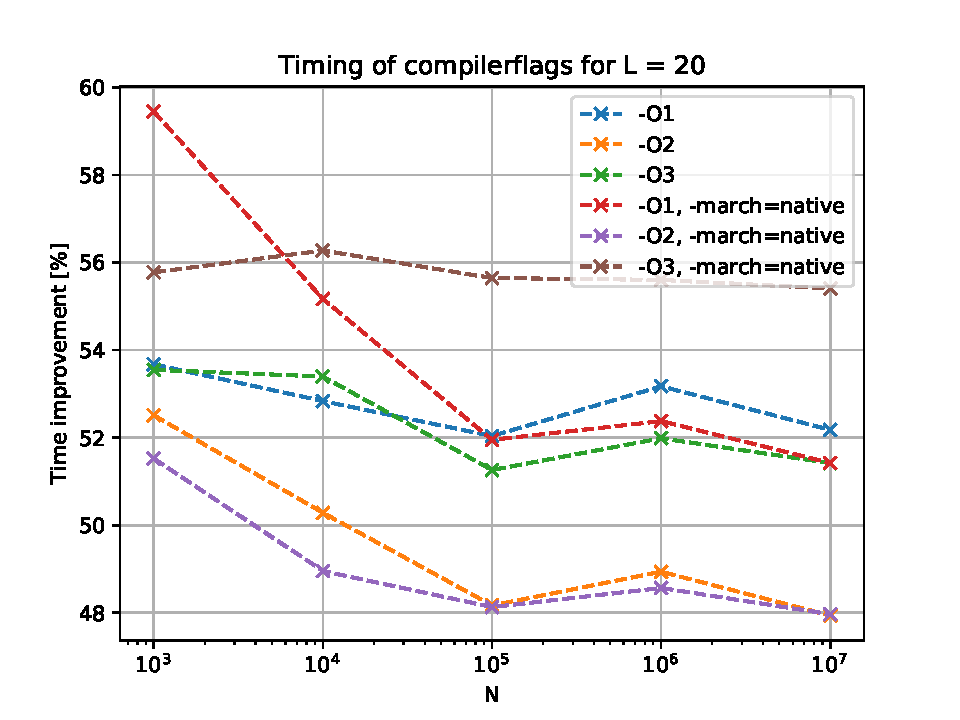
\includegraphics[width=\columnwidth]{../data/benchmark.pdf}
	\caption{Time improvement in percentage of various compiler optimization flags for a \(20\times 20\) lattice with \(8\) evenly spaced values of \(T \in [2.20, 2.35]\). All results are achieved with parallelized runs with \(8\) threads (one value of \(T\) per thread)} \label{fig:benchmark_compiler_flags}
\end{figure}



\subsection{Simulation with a $2\times 2$ lattice} \label{sec:IV:B}

We simulated a $2 \times 2$ lattice to compare with the analytical results found in section \hyperref[sec:II:A:i]{II.A.1}. In these simulations we recorded the energy and magnetization per spin in each Monte Carlo sweep in order to observe how they develop, and how the values derived from them also develop as a function of the amount of sweeps performed. We have plotted the energy, absolute of magnetization, heat capacity and magnetic susceptibility as functions of the amount of sweeps performed, and these plots can be seen in figures \ref{fig:t10_2x2_energy_magnetization} and \ref{fig:t10_2x2_heat_capacity_susceptibility}. The analytic values found in equations \eqref{eq:2x2_energy}, \eqref{eq:2x2_abs_magnetization}, \eqref{eq:2x2_heat_capacity}, and \eqref{eq:2x2_susceptibility} are also plotted for comparison. We also calculated errors and relative errors in the final values for all of these quantities and also the absolute error for the mean magnetization. These are listed in table \ref{table:t10_2x2_errors}. The errors are the differences between the numerical values and the analytical values.

\begin{figure}[H]
\centering
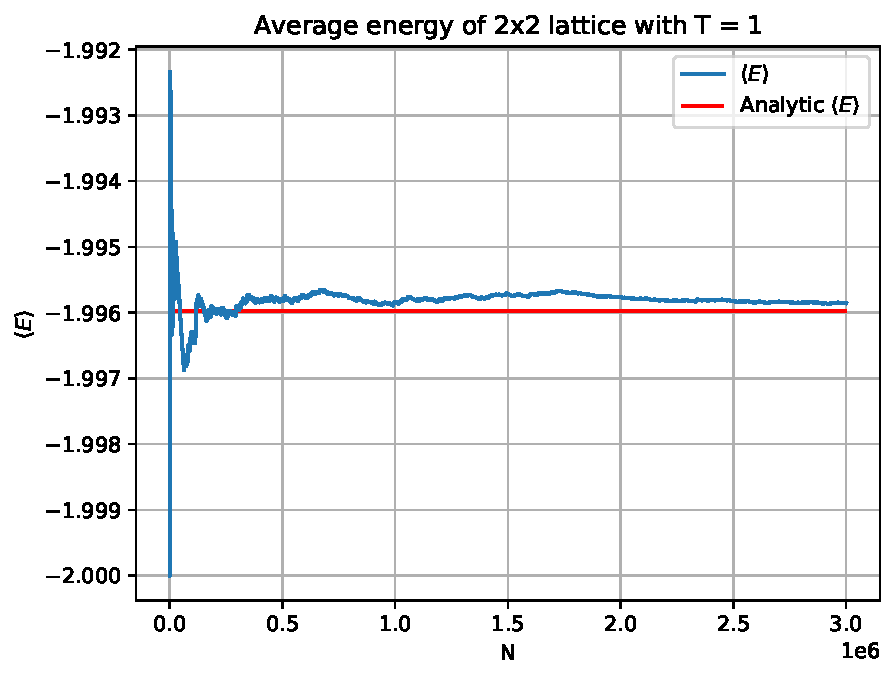
\includegraphics[width=\columnwidth]{../data/t10-2x2-E.pdf}
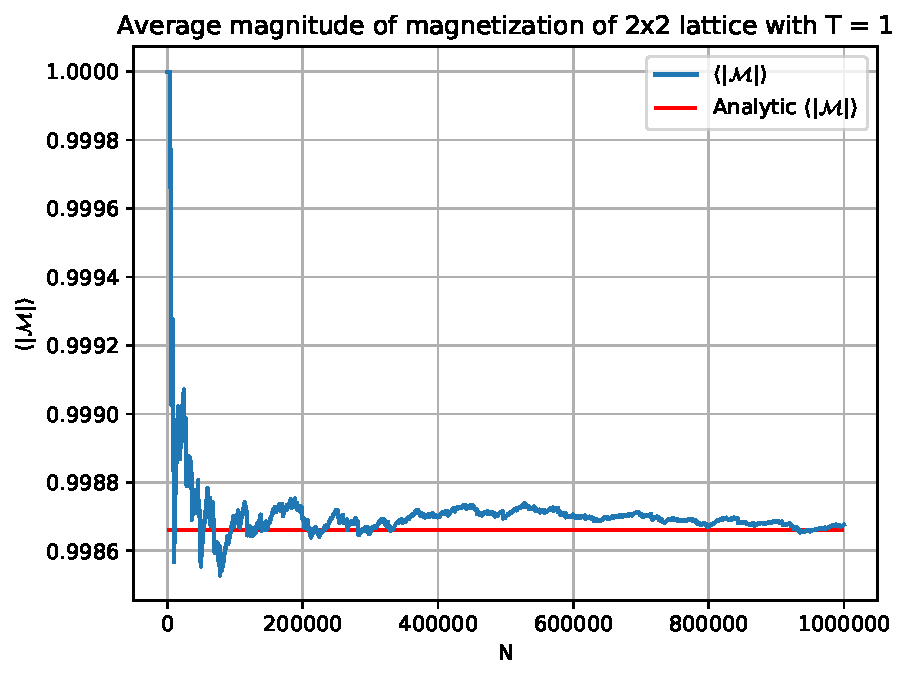
\includegraphics[width=\columnwidth]{../data/t10-2x2-|M|.pdf}
\caption{This figure contains plots of the mean energy per spin and the mean absolute value of the magnetization per spin as functions of the amount of Monte Carlo sweeps performed for a simulation with a $2\times 2$ lattice and with temperature $T=1$ (in units of $k_B T/J$). The plots also contain the analytic values for these as given in equation \eqref{eq:2x2_energy} and \eqref{eq:2x2_abs_magnetization}.} \label{fig:t10_2x2_energy_magnetization}
\end{figure}

\begin{figure}[H]
\centering
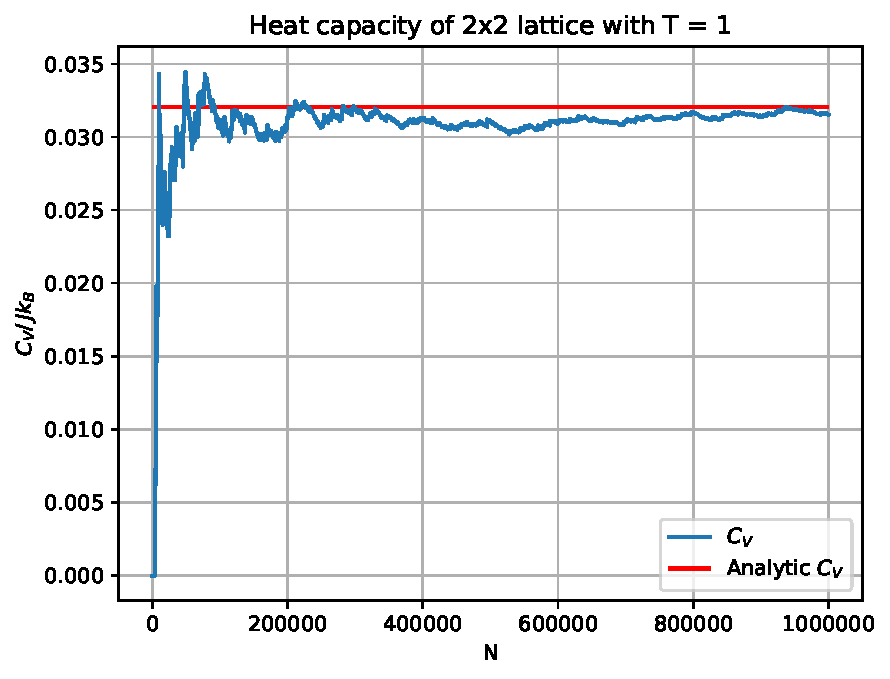
\includegraphics[width=\columnwidth]{../data/t10-2x2-Cv.pdf}
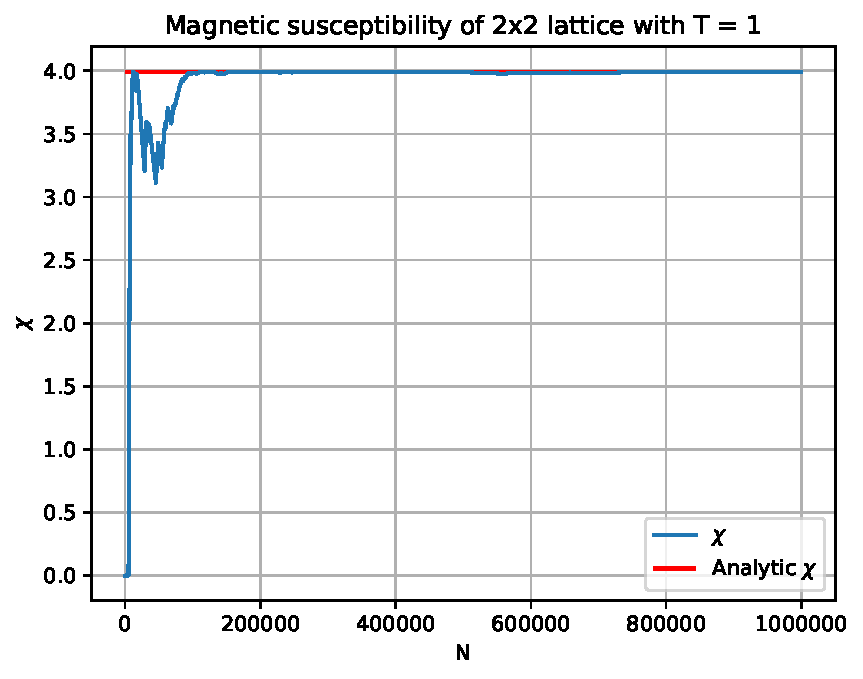
\includegraphics[width=\columnwidth]{../data/t10-2x2-Xi.pdf}
\caption{This figure contains plots of the heat capacity per spin and the magnetic susceptibility per spin as functions of the amount of Monte Carlo sweeps performed for a simulation with a $2\times 2$ lattice and with temperature $T=1$ (in units of $k_B T/J$). The plots also contain the analytic values for these as given in equation \eqref{eq:2x2_heat_capacity} and \eqref{eq:2x2_susceptibility}.} \label{fig:t10_2x2_heat_capacity_susceptibility}
\end{figure}

\begin{table}[H]
\centering 
\caption{This table contains errors in the numerically calculated values of the mean energy $\langle E \rangle$, mean magnetization $\langle \mathcal{M} \rangle$, mean absolute of the magnetization $\langle |\mathcal{M}| \rangle$, heat capacity $C_V$ and magnetic susceptibility $\chi$ (all per spin) for a $2\times 2$ lattice with $T=1$ /in units of $k_BT/J$) after $10^6$ Monte Carlo sweeps. The numerically calculated values are compared to their analytic counterparts as they are given in equations \eqref{eq:2x2_energy}, \eqref{eq:2x2_abs_magnetization}, \eqref{eq:2x2_heat_capacity}, and \eqref{eq:2x2_susceptibility}. Also note that the analytic value for the mean magnetization is zero, and thus there is no relative error listed as it is undefined.} \label{table:t10_2x2_errors}
\begin{tabular}{|c|c|c|}
\hline
Value & Error & Relative error \\
\hline
$\langle E \rangle$ & \num{-6.991e-05} & \num{3.503e-05} \\
\hline
$\langle \mathcal{M} \rangle$ & \num{-5.221e-03} & - \\
\hline
$\langle |\mathcal{M}| \rangle$ & \num{1.527e-05} & \num{1.529e-05} \\
\hline 
$C_V$ & \num{-5.535e-04} & \num{1.726e-02} \\
\hline
$\chi$ & \num{-8.811e-06} & \num{2.207e-06} \\
\hline
\end{tabular}
\end{table}

\subsection{Simulations with a $20 \times 20$ lattice} \label{sec:IV:C}

In order to evaluate the stability and convergence of our solver we simulated a $20 \times 20$ lattice of spins with temperatures $T = 1$ and $T = 2.4$ (in units of $k_B T/J$). We ran these simulations with both an ordered intial state (all spins pointing up) and a disordered initial state (randomized spin configuration). Plots of the average energy, absolute of the magnetization, and the number of accepted configurations as functions of the amount of Monte Carlo cycles performed in the simulations with $T=1$ can be seen in figures \ref{fig:20x20-T1.0-energy}, \ref{fig:20x20-T1.0-absolute_magnetization} and \ref{fig:20x20-T1.0-Nconf} respectively. Similar plots for the simulations with $T=2.4$ can be seen in figures \ref{fig:20x20-T2.4-energy}, \ref{fig:20x20-T2.4-absolute_magnetization}, and \ref{fig:20x20-T2.4-Nconf}. We also calculated the probability distributions for the energy in these simulations and they can be seen in figure \ref{fig:20x20-T1.0-PE} for $T=1$ and figure \ref{fig:20x20-T2.4-PE} for $T=2.4$. The probability distributions were calculated by binning the the energy values recorded during the simulations and normalizing the results. This was done using Matplotlib's histogram function. A slightly modified normal distribution is also plotted on top of the plots of the probability distribution for $T=2.4$. In order to get the peaks to be approximately similar, it was necessary to multiply the normal distribution by a constant $2.2$. 


\begin{figure}[H]
\centering
\includegraphics[width=\columnwidth]{{"../data/ordered initial spin.-t1.0-20x20-E"}.pdf}
\includegraphics[width=\columnwidth]{{"../data/disordered initial spin.-t1.0-20x20-E"}.pdf}
\caption{This figure contains plots of mean energy as a function of amount of Monte Carlo cycles performed for simulations with a $20\times 20$ lattice and temperature $T=1$ (in units of $k_B T/J$). The first plot shows the development of the energy when the initial state is ordered (all spins pointing up) and the second plot shows the energy when the initial state is disordered (randomized spin configuration).} \label{fig:20x20-T1.0-energy}
\end{figure} 

\begin{figure}[H]
\centering
\includegraphics[width=\columnwidth]{{"../data/ordered initial spin.-t1.0-20x20-|M|"}.pdf}
\includegraphics[width=\columnwidth]{{"../data/disordered initial spin.-t1.0-20x20-|M|"}.pdf}
\caption{This figure contains plots of the mean absolute of the magnetization as a function of amount of Monte Carlo cycles performed for simulations with a $20\times 20$ lattice and temperature $T=1$ (in units of $k_B T/J$). The first plot shows the development of the magnetization when the initial state is ordered (all spins pointing up) and the second plot shows the magnetization when the initial state is disordered (randomized spin configuration).} \label{fig:20x20-T1.0-absolute_magnetization}
\end{figure} 

\begin{figure}[H]
\centering
\includegraphics[width=\columnwidth]{{"../data/ordered initial spin.-t1.0-20x20-Nconf"}.pdf}
\includegraphics[width=\columnwidth]{{"../data/disordered initial spin.-t1.0-20x20-Nconf"}.pdf}
\caption{This figure contains plots of the total amount of accepted configurations as a function of amount of Monte Carlo cycles performed for simulations with a $20\times 20$ lattice and temperature $T=1$ (in units of $k_B T/J$). The first plot shows the amount of accepted configurations when the initial state is ordered (all spins pointing up) and the second plot shows amount of accepted configurations when the initial state is disordered (randomized spin configuration).} \label{fig:20x20-T1.0-Nconf}
\end{figure}

\begin{figure}[H]
\centering
\includegraphics[width=\columnwidth]{{"../data/ordered initial spin.-t1.0-20x20-PE"}.pdf}
\includegraphics[width=\columnwidth]{{"../data/disordered initial spin.-t1.0-20x20-PE"}.pdf}
\caption{This figure contains plots of the numerically calculated probability distribution of the energy with a $20\times 20$ lattice and temperature $T=1$ (in units of $k_B T/J$). The first plot shows the probability distribution when the initial state is ordered (all spins pointing up) and the second plot shows the probability distribution when the initial state is disordered (randomized spin configuration).} \label{fig:20x20-T1.0-PE}
\end{figure} 


\begin{figure}[H]
\centering
\includegraphics[width=\columnwidth]{{"../data/ordered initial spin.-t2.4-20x20-E"}.pdf}
\includegraphics[width=\columnwidth]{{"../data/disordered initial spin.-t2.4-20x20-E"}.pdf}
\caption{This figure contains plots of mean energy as a function of amount of Monte Carlo cycles performed for simulations with a $20\times 20$ lattice and temperature $T=2.4$ (in units of $k_B T/J$). The first plot shows the development of the energy when the initial state is ordered (all spins pointing up) and the second plot shows the energy when the initial state is disordered (randomized spin configuration).} \label{fig:20x20-T2.4-energy}
\end{figure} 

\begin{figure}[H]
\centering
\includegraphics[width=\columnwidth]{{"../data/ordered initial spin.-t2.4-20x20-|M|"}.pdf}
\includegraphics[width=\columnwidth]{{"../data/disordered initial spin.-t2.4-20x20-|M|"}.pdf}
\caption{This figure contains plots of the mean absolute of the magnetization as a function of amount of Monte Carlo cycles performed for simulations with a $20\times 20$ lattice and temperature $T=2.4$ (in units of $k_B T/J$). The first plot shows the development of the magnetization when the initial state is ordered (all spins pointing up) and the second plot shows the magnetization when the initial state is disordered (randomized spin configuration).} \label{fig:20x20-T2.4-absolute_magnetization}
\end{figure} 

\begin{figure}[H]
\centering
\includegraphics[width=\columnwidth]{{"../data/ordered initial spin.-t2.4-20x20-Nconf"}.pdf}
\includegraphics[width=\columnwidth]{{"../data/disordered initial spin.-t2.4-20x20-Nconf"}.pdf}
\caption{This figure contains plots of the total amount of accepted configurations as a function of amount of Monte Carlo cycles performed for simulations with a $20\times 20$ lattice and temperature $T=2.4$ (in units of $k_B T/J$). The first plot shows the amount of accepted configurations when the initial state is ordered (all spins pointing up) and the second plot shows amount of accepted configurations when the initial state is disordered (randomized spin configuration).} \label{fig:20x20-T2.4-Nconf}
\end{figure}

\begin{figure}[H]
\centering
\includegraphics[width=\columnwidth]{{"../data/ordered initial spin.-t2.4-20x20-PE"}.pdf}
\includegraphics[width=\columnwidth]{{"../data/disordered initial spin.-t2.4-20x20-PE"}.pdf}
\caption{This figure contains plots of the numerically calculated probability distribution of the energy with a $20\times 20$ lattice and temperature $T=2.4$ (in units of $k_B T/J$). The first plot shows the probability distribution when the initial state is ordered (all spins pointing up) and the second plot shows the probability distribution when the initial state is disordered (randomized spin configuration). Both plots include a normal distribution as well, which have mean and variance equal to that of the energy.} \label{fig:20x20-T2.4-PE}
\end{figure} 



\subsection{Simulations with larger lattice sizes} \label{sec:IV:D}

% Creating variables for simulation specs so we do not have to change them everywhere if we change them later
\newcommand{\tempsteps}{8}
\newcommand{\tempmin}{2.20}
\newcommand{\tempmax}{2.35}
\newcommand{\nmax}{10^7}

We ran simulations with lattice sizes $40\times 40$, $60 \times 60$, $80 \times 80$ and $100 \times 100$ in the temperature range $T\in[\tempmin ,\tempmax ]$ (in units of $k_B T/J$) in order to look for signs of a phase transition. All the simulations were ran with $N=\nmax$ Monte Carlo sweeps. A phase transition should occur at the critical temperature. The analytical critical temperature for an infinite lattice is given in \eqref{eq:crit_temperature_analytical} and the critical temperatures for different lattice dimensions $L$ is related to the one for an infinite lattice as shown in \eqref{eq:crit_temperature_finite_lattice}. The critical temperatures measured for different lattice sizes should always be larger than the one for an infinite lattice, and so we selected the temperature interval to be such that the critical temperature for an infinite lattice is slightly less than the middle value of the interval. We chose to use $\tempsteps$ temperature steps. The calculated mean energy per spin as a function of temperature can be seen in figure \ref{fig:ph-energy}, the mean magnetization and mean absolute of the magnetization as functions of temperature can be seen in figure \ref{fig:ph-magnetization}, and the heat capacity and susceptibility as functions of temperature can be seen in \ref{fig:ph-heat-capacity-susceptibility}. We estimated the critical temperatures using the methods outlined in section \hyperref[sec:III:A.iv]{III.A.4}, and the values found are listed in table \ref{table:crit_temps}. The relative error of the numerically calculated critical temperature for an infinite lattice compared to the analytical one was found to be \num{3.78e-06}.


\begin{figure}[H]
\centering
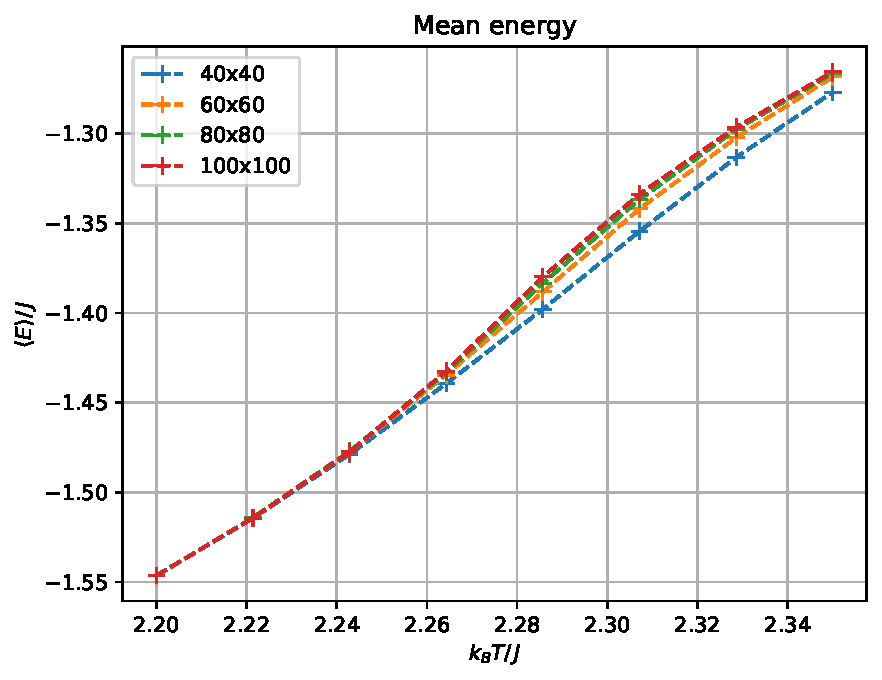
\includegraphics[width=\columnwidth]{../data/phase-transition-E.pdf}
\caption{This figure contains a plot of the mean energy per spin as a function of temperature from simulations with lattice sizes as indicated by the legend in the plot.} \label{fig:ph-energy}
\end{figure}

\begin{figure}[H]
\centering
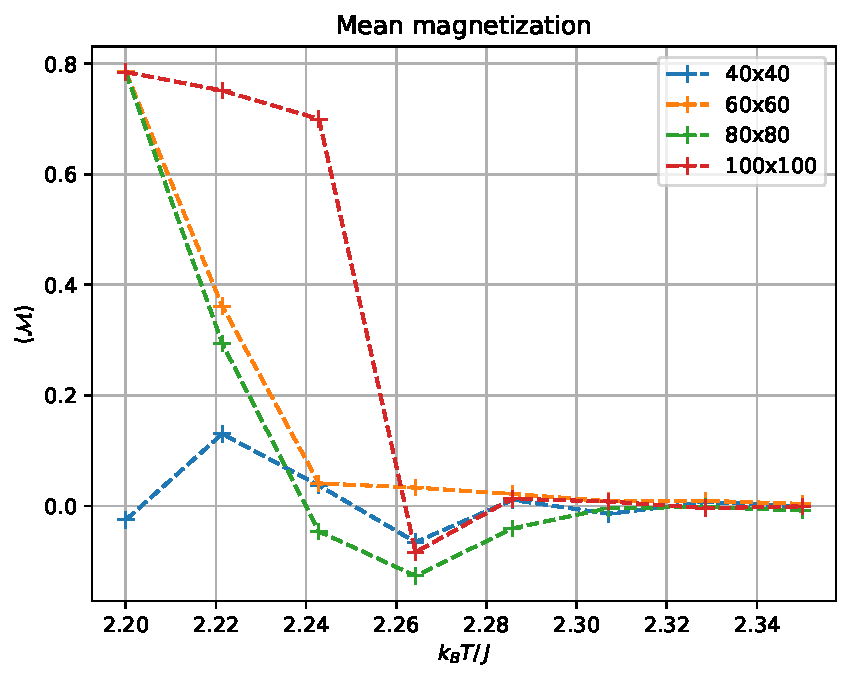
\includegraphics[width=\columnwidth]{../data/phase-transition-M.pdf}
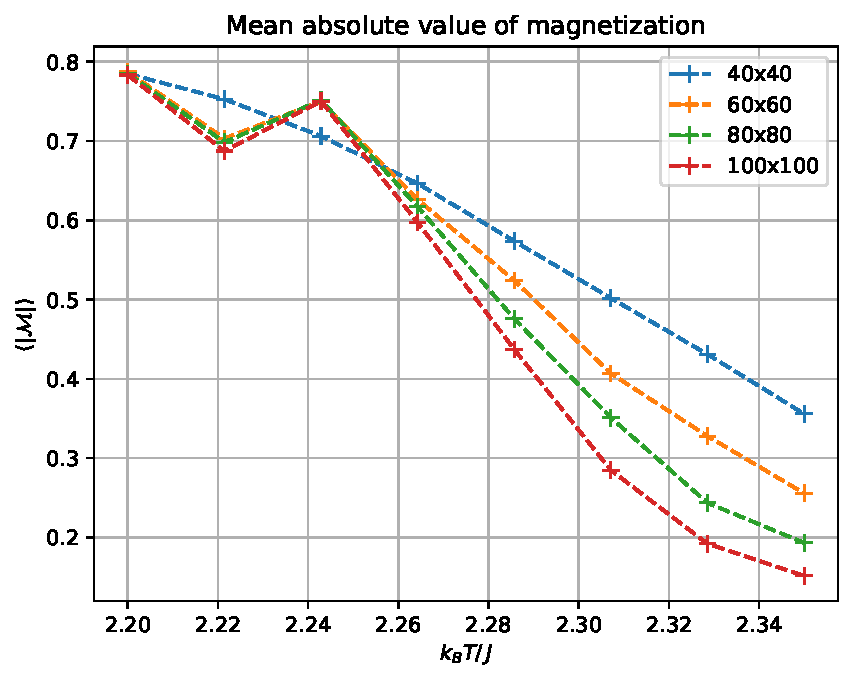
\includegraphics[width=\columnwidth]{../data/phase-transition-|M|.pdf}
\caption{This figure contains plots of the mean magnetization per spin and mean absolute of the magnetization per spin as functions of temperature from simulations with lattice sizes as indicated by the legend in the plot.} \label{fig:ph-magnetization}
\end{figure}

\begin{figure}[H]
\centering
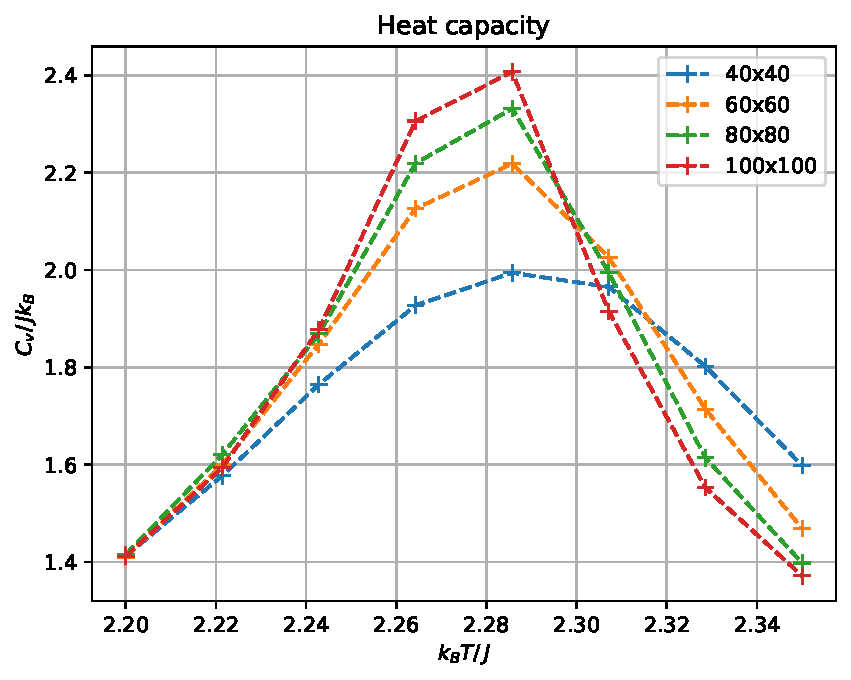
\includegraphics[width=\columnwidth]{../data/phase-transition-Cv.pdf}
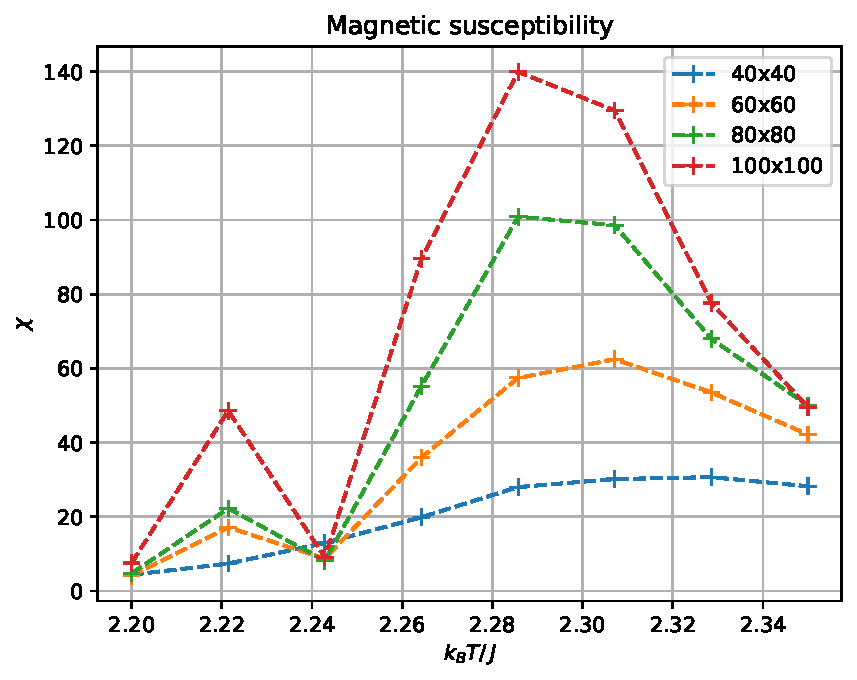
\includegraphics[width=\columnwidth]{../data/phase-transition-Xi.pdf}
\caption{This figure contains plots of the heat capacity per spin and magnetic susceptibility per spin as functions of temperature from simulations with lattice sizes as indicated by the legend in the plot.} \label{fig:ph-heat-capacity-susceptibility}
\end{figure}

\begin{table}[H]
\centering
\caption{This table contains numerically calculated critical temperatures $T_C(L)$ for lattice sizes $L \times L$. The critical temperature for an infinite lattice $T_C(L=\infty)$ is estimated from the other values using equation \eqref{eq:crit_temperature_finite_lattice}, and has a relative error of \num{3.78e-06} compared to the analytical result listed in \eqref{eq:crit_temperature_analytical}.} \label{table:crit_temps}
\begin{tabular}{|c|c|c|c|c|c|}
\hline
$L$ & 40 & 60 & 80 & 100 & $\infty$ \\
\hline
$T_C(L)$ & 2.307 & 2.296 & 2.286 & 2.286 & $2.269\pm 0.004$ \\
\hline
\end{tabular}
\end{table}


\newpage

\section{Discussion} \label{sec:V}

We have implemented a solver for a two-dimensional Ising model of spin interactions, in a square lattice with no external field, using the Metropolis algorithm. Using this solver we have simulated this model at several temperatures and lattice sizes, and in this section we will discuss the results presented in the previous sections.

\subsection{Benchmark, timings and parallelization} \label{sec:V:A}
From the results in table \hyperref[table:benchmark_parallel]{II}, we se that parallelizing our metropolis simulation of the ising model by simulating one temperature value per thread, gives a reduction in time spent of approximately \(85\%\) over the serialized version. Furthermore, the time spent on the parallelized version is approximately halved by using the same compiler optimization flags as the serialized version. From figure \ref{fig:benchmark_compiler_flags} we see that the combination of the -O3 and -march=native compiler flags offered the best performance increase for \(10^{4}\) or more Monte Carlo cycles with the parallelized implementation. While the -O1, -O2, and -O3 optimization flags offer general optimization, the -march=native flag tells the compiler (GCC v9.3.0) to attempt optimizations that are specific to the system's CPU architecture. Thus, the benefit of the -march=native flag is highly dependent on the choice of CPU, and may not behave as expected when also using OpenMP or other forms of parallelization.

As discussed in section \ref{sec:III:a:iii}, our simulation of the Ising model is parallelized by temperature values, running a simulation of one temperature per thread, and by lattice dimension \(L\), running \(8\) threads per value of \(L\). While each thread for a given \(L\) will perform the same number of Monte Carlo cycles and lattice sweeps. The number of lattice sweeps varies significantly for differing values of \(L\). Thus our workload is uneavenly distributed between threads when running concurrent simulations for multiple values of \(L\).

We considered parallelizing the Monte Carlo cycles, and allowing the temperatures and values of \(L\) to be handled in series. While such an alternate parallelization would have more evenly distributed work between threads, it would also lead to more overhead from parallelization, as the multi-thread region would be created and closed for each temperature and value of \(L\). Having relatively little work per thread and repeated initialization of a parallel region could lead to diminishing returns, as the overhead of creating and closing the parallel region might balance out the performance gained from having multiple threads.

Another potential benefit of our choice of parallelization is that once the simulations with smaller \(L\) finishes, the associated cores will reduce their power consumption and heat output, allowing the remaining active cores to operate at a higher sustained clock speed. While this might not be particularly beneficial for server grade CPUs with a high number of cores and relatively low maximum clock speeds, it might be noticeably beneficial on consumer grade CPUs, such as the one used in this report, that have relatively few cores and higher maximum clock speeds. We leave investigating the potential benefit of higher clock speeds versus amount of threads to future research.

\subsection{Simulation with a $2\times 2$ lattice} \label{sec:V:B}

The results from this simulation can be seen in section \hyperref[sec:IV:B]{IV.B}. As expected we see (in figures \ref{fig:t10_2x2_energy_magnetization} and \ref{fig:t10_2x2_heat_capacity_susceptibility}) that the mean energy, absolute of the magnetization, heat capacity and susceptibility all stabilize around the expected values we derived in section \hyperref[sec:II:A:i]{II.A.1} after a sufficient amount of Monte Carlo sweeps ($N$ in the plots) have been performed. In general we see that all the values start to get close to their expected values after about $10^5$ sweeps, and that they are fairly stable after \num{2e5} sweeps. At first glance it may seem like the magnetic susceptibility is much more stable than the energy, heat capacity, and absolute of the magnetization, but that is not really the case, as the scale of the vertical axis in the plot of the magnetic susceptibility is much larger than in the other plots.

We also calculated the error (difference between numerically calculated and analytical values) and the relative errors in the final values of the energy, magnetization, absolute of the magnetization, heat capacity and mangetic susceptibility. These results can be seen in table \ref{table:t10_2x2_errors}. The errors are not all that interesting, as none of them are very large. What is interesting though, is that they are all, except for the absolute of the magnetization, smaller than the analytical values. This is most likely an artifact of the initial configuration of the system (in this simulation the initial configuration was all spins pointing up). As most of the relative errors are also very small, we can conclude that the numerical values converge as expected. One notable exception here is the heat capacity, where there is a relative error of almost 2\%. An error such as this is significant, but we must also take into account that the system here is very small, and is thus fairly prone to numerical error as we discussed in section \hyperref[sec:III:C]{III.C}. 

We also chose to use this system as a unit-test for our implementation, and as it is desirable to compare the numerical and analytical values for all of the quantities measured we also include a comparison of the heat capacity. As the relative error in the heat capacity is significantly larger than the other quantities the tolerance in this test also needs to be larger in order for the test to pass. In general it is bad practice to adjust the test to the results, but due to the nature of these simulations it is necessary to first attempt to quantify the size of the numerical errors we make in order to determine what a good selection of tolerance is. Therefore we chose to first 
test that the results behaved as expected, and then formulate the unit-test to make sure that nothing breaks after we have verified that the solver works as it should.

\subsection{Simulations with a $20 \times 20$ lattice} \label{sec:V:C}

We ran simulations with a $20 \times 20$ lattice with four different sets of initial configration and temperature. The results from these simulations can be seen in section \hyperref[sec:IV:C]{IV.C}. For both disordered and ordered initial configuration with $T=1$ (in units of $k_B T/J$), we see that the energy and the magnitude of the magnetization are fairly stable after $N=\num{4e5}$ Monte Carlo sweeps (see figures \ref{fig:20x20-T1.0-energy} and \ref{fig:20x20-T1.0-absolute_magnetization}), so it is apparent that they converge slower than in the $2 \times 2$ case. With $T=2.4$ the convergence is even slower (see figures \ref{fig:20x20-T2.4-energy} and \ref{fig:20x20-T2.4-absolute_magnetization}), and it seems that about $N=\num{5e5}$ sweeps are necessary for the magnetization to be stable. This indicates that for temperatures closer to the critical temperature we might need more Monte Carlo sweeps in order to provide reliable results. In general we expect the behaviour of these quantities to be more drastic closer to the critical temperature. As $T=2.4$ is closer to the analytical critical temperature for an infinite lattice given in \eqref{eq:crit_temperature_analytical} than $T=1$ we assume this to be the case for the critical temperature of this lattice size as well. We have, however, not ran simulations for enough temperatures with this lattice size in order to provide any kind of reliable estimate as to what the critical temperature actually is. 

Every time a spin was flipped during these simulations, we counted this as a new accepted configuration. Plots of this count of accepted configurations can be seen in figure \ref{fig:20x20-T1.0-Nconf} for $T=1$, and in figure \ref{fig:20x20-T2.4-Nconf} for $T=2.4$. In general we see that many more configurations are accepted for the higher temperature. This is not unexpected, as the probability for the change of configuration that we use is the Boltzmann distribution. When $T$ is larger the boltzmann factor is larger for disfavourable energy changes, meaning that we are more likely to accept configurations with disfavourable energy changes. In general this means that more new configurations will be accepted. The number of accepted configurations as a function of the amount of Monte Carlo sweeps is very nearly linear (the increase decreases very slightly for larger $N$), and so we decided to provide logarithmic plots as these better highlight the differences in accepted configurations between the two temperatures. 

An attempt was also made to estimate the probability distribution of the energy values that were calculated in figures \ref{fig:20x20-T1.0-PE} and \ref{fig:20x20-T2.4-PE} for $T=1$ and $T=2.4$ respectively. As the generation of these energy values are pseudo-random we expect (as given by the central limit theorem) that they will behave approximately according to a normal distribution with the same mean and variance as observed in the energy, but with some caveats. These caveats prove to be significant. The lattice size we are operating with are finite, and this means that there are only a finite amount of possible energies. This can clearly be seen in both the estimated probability distribution. Also there are lower and upper limits to the energies, so we also expect the probability distributions to be skewed either to the right or the left depending on which limit we are closer to. For $T=1$ the estimated probability distribution is heavily skewed, as the lowest allowed energy of $-2J$ per spin is the the most likely configuration. The finite allowed energy values can also be seen as there are "holes" between the bins. Thus this distribution does not look like a normal distribution at all, and we have omitted the plotting of a comparison normal distribution. 

The plots showing the probability distribution for $T=2.4$ are more interesting, however. These clearly take the shape of the normal distribution, with a slight skew. We also see some holes between bins where there are no measured energy values as expected. Due to these holes the normal distribution that was plotted had to be multiplied by a factor of approximately $2.2$ in order for the peaks to be of similar size. The normal distribution plotted has the mean and variance that we measured for the energy, and as the shape of the distributions are as similar as they are, we can conclude that the probability distribution of the energies behaves as expected.

We also need to discuss the differences between ordered and disordered initial spin configurations. The energy and magnetizations seem to converge fairly quickly in all cases, and thus we can conclude that which initial configuration we choose is not of any major consequence. However, we can see that for $T=1$ the ordered initial spin configurations is closer to the equillibrium state, as the energy and magnetization needs to change less in order to reach their stable values in general. So in cases where the temperature is low it should almost always be better to use an ordered initial spin state. For larger temperatures the ordered initial spin configurations will never really be close to the equillibrium state, but the disordered initial spin configuration might be. This does not always mean that the disordered initial spin configuration is better in terms of convergence in these cases, as one would need to calculate the probability of it being closer to the equillibrium state than the ordered initial spin configuration, which is difficult. However, from a physical point of view, a disordered initial spin state that is then eqillibrated is more likely than a fully ordered initial spin state. Thus we elect to use the disordered initial spin configuration in general, even though the ordered initial spin configuration might be closer to the equillibrium state.



\subsection{Simulations with larger lattice sizes} \label{sec:V:D}

We also ran our solver for lattice sizes $40\times 40$, $60\times 60$, $80 \times 80$ and $100 \times 100$ in a temperature interval $T\in [\tempmin,\tempmax]$ (in units of $k_B T/J$) with $\tempsteps$ steps in temperature from the smallest to the largest value. The results are shown in section \hyperref[sec:IV.D]{IV.D}. The mean energy per spin as seen in figure \ref{fig:ph-energy} increases with the temperature $T$ for all lattice sizes. For $T=2.2$ we can see that the mean energy per spin is roughly similar for all lattice sizes, but as $T$ increases they start to split apart. At roughly $T=2.3$ this split seems to reach a maximum, and the energy per spin for the different lattice sizes seems to come back together. None of this is surprising. We expect there to be some difference between the different lattice sizes, and unsurprisingly it reaches a maximum in the area around where we expect the critical temperature to be when we compare with the analytical result for an infinite lattice \eqref{eq:crit_temperature_analytical} using equation \eqref{eq:crit_temperature_finite_lattice}.

The mean magnetization seen in figure \ref{fig:ph-magnetization} is difficult to extract any useful information from. If all spins are flipped the energy of the system remains the same, while the magnetization changes sign. As the probability that governs the development of the system (the Boltzmann distribution \eqref{eq:boltzmann_dist}) is independent of the magnetization, but dependent of the energy, this means that we might see wildly varying magnetizations. Thus it is more of interest to look at the mean magnitude of the magnetization, which can be seen in the second plot in the same figure. The fact the magnetization is decaying increasingly until it reaches a point where it starts to stabilize again is a sign of a phase transition occuring. When the system moves from an ordered to a disorded state as it should at higher temperature we expect the magnetization to approach zero, and this is the case in both of these plots. The mean magnetization shows clearer behvaiour of getting closer to zero above the critical temperature (which should be smaller the larger the lattice dimensions are) than the mean magnitude of the magnetization. This is not unexpected, as there will be small oscillations around the stable value for the magnetization. When taking the mean these add up to zero in the case of the magnetization itself, but they will add up to a positive value for the mean magnitude of the magnetization. All in all these plots seem to indicate a phase transition, as we see a steep decline in the magnetization as expected from the power law behaviour outlined in section \hyperref[sec:II:A:ii]{II.A.2} (see equation \eqref{eq:power_law_magnetization_per_spin}). 

The heat capacity and magnetic susceptibility (shown in figure \ref{fig:ph-heat-capacity-susceptibility}) both show clear signs of a phase transition  occuring. These are expected to peak around the critical temperature, and we can see they reach a peak for all the lattice sizes simulated, but that the peak is smaller the smaller the lattice size is. This is all as expected according to the power law behaviour that we expect to see. In order to estimate the critical temperatures we identified the temperature at which these two quantities peaked for all the lattice sizes, and averaged them. We can clearly see from the plots shown that if we used only the heat capacity our results would be very interesting as it peaks at the same temperature value for all the lattice sizes. The magnetic susceptibility however, does not. In general averaging the two temperature values obtained from these peaks for each lattice sizes lowers the expected error in the result. 

By doing this we found estimates of the critical temperatures $T_C(L)$ at difference lattice sizes $L \times L$, which are listed in table \ref{table:crit_temps}. As they are expected to behave as a first degree polynomial of $1/L$ (according to equation \eqref{eq:crit_temperature_finite_lattice} with $\nu=1$) with $T_C(L=\infty)$ as the constant term, we were able to fit the values to this polynomial using NumPy's \verb+polyfit()+ function. This also provides us with the uncertainty in the constant in the fitting by ways of the covariance matrix, and so we found the critical temperature in the thermodynamical limit to be $T_C(L=\infty) = 2.269 \pm 0.004$. This overlaps with the analytical result given in \eqref{eq:crit_temperature_analytical}, and the obtained value itself was found to have a relative error of only \num{3.78e-06}. From looking at these results it is clear that our solver is working as intended, and that the phase transition occurs as expected, at the temperatures that they are expected to occur at. Our solver seems to provide reliable results, and can thus be used for further research with this model. 


\subsection{Final note on the errors in the simulations} \label{sec:V:E}

In general our results present very few signs of there being large numerical errors. It seems that as long as we let the system equillibrate properly, and operate with large enough lattice sizes, that the numerical errors in the results are very small. Relating this to our discussions in section \hyperref[sec:III:C]{III.C} this seems to indicate that as expected, none of the potential error sources play a huge part. From looking at our results, we can be fairly certain that our random number generator is not causing any issues, and that there is no loss of precision due to the lattice sizes being too large compared to the amount of Monte Carlo sweeps. The latter source of errors is one that we likely do not encounter due to limitations on the scale of simulations that we can run. 

For future research, with more computational resources available, this will become significant and an adapatation must be done, or else the errors in the results will be significant. Changing the method of calculating the averages will most likely involve adding floating point operations to each sweep, and with this there is a possibility for the truncation error in these to propagate and add a more significant contribution to the errors in the results. Thus the more desirable method of increasing the scaling options of the simulations is simply to use larger data types to store the values. By changing the variables from doubles to 16 byte long doubles we can double the amount of significant digits that they contain. This would also increase the amount of Monte Carlo sweeps that we can have before there is loss of precision by a order of magnitude equal to the amount of significant digits added by this change of variable type. Thus we recommend for future research using similar methods for even larger lattice sizes to consider the effects of this interaction between lattice size and amount of Monte Carlo sweeps, and from that picking the data type that is best suited to the simulation. 

\clearpage



\section{Conclusion} \label{sec:VI}

We have implemented a solver for the Ising Model in two dimensions, with a square lattice and no exeternal field, using the Metropolis algorithm. This implementation was used to simulate this system for various lattice sizes and temperatures. By parallelizing our simulations of multiple temperatures for multiple lattice sizes, we were able to achieve an approximately \(85\%\) increase in performance over the serialized version of our code. Using parallelization in combination with compiler optimization flags, we achieved another approximately \(55\%\) performance increase over the unoptimized parallel implementation.

Numerical results from our` simulations, such as mean energy, mean magnetization, mean magnitude of the magnetization, heat capacity, and magnetic susceptibility were all compared to their analytical counterparts, and in general we found good agreement between these. This indicates that our implementation generates correct results, within limitations on lattice size and amount of Monte Carlo sweeps performed. In general a certain amount of sweeps is necessary for the solution to converge, and smaller lattice sizes can cause significant contributions to the numerical errors, which we found to be the case at least somewhat. We also expected there to be an upper limit on the amount of Monte Carlo sweeps that can be performed for a given lattice size before we start to lose significant digits during the calculation of the results, but this limit was not encountered in our simulations. All in all, nothing was found that indicates that our implementation does not work as it should.

For larger lattice sizes we expect to see phase transition behaviour around a critical temperature. When we simulated for different lattice sizes, we were able to estimate the critical temperature of the system at some of these lattice sizes and from these results estimate the critical temperature in the thermodynamical limit $T_C(L=\infty) = 2.269 \pm 0.004$. This overlaps with the analytical value of $T_C(L=\infty) = 2/\ln(1 + \sqrt{2})$, and has a relative error \num{3.78e-06} from the value itself when all digits produced are taken into account.

Through tests of the convergence of the results, we found that how many Monte Carlo sweeps that are necessary for the system to equilibrate depends on the temperature and the lattice size. In general the amount of sweeps necessary for the solution to converge increases both when the lattice size increases, and when the temperature gets closer to the critical temperature. 

\onecolumngrid
\bibliography{kilder.bib}{}
\newpage
\twocolumngrid

\appendix
\section{Source code} \label{A}
All code for this report was written in C++ and Python 3.6, and the complete set of files can be found at:

\url{https://github.com/eivinsto/FYS3150_Project_4.git}.

\cprotect\subsection{\verb+ising_metropolis.hpp+} \label{A.1}

Header file containing definitions for the \verb+IsingMetropolis+ class, which is used to run the simulations. The file can be found at:

\url{https://github.com/eivinsto/FYS3150_Project_4/blob/main/src/ising_metropolis.hpp}

\cprotect\subsection{\verb+ising_metropolis.cpp+} \label{A.2}

Source file containing the methods and constructors belonging to the \verb+IsingMetropolis+ class. The file can be found at:

\url{https://github.com/eivinsto/FYS3150_Project_4/blob/main/src/ising_metropolis.cpp}

\cprotect\subsection{\verb+main.cpp+} \label{A.3}

Main program which can operate the simulations run in the \verb+IsingMetropolis+ class using command line arguments. The file can be found at:

\url{https://github.com/eivinsto/FYS3150_Project_4/blob/main/src/main.cpp}

\cprotect\subsection{\verb+python.py+} \label{A.4}

Python script that automates the simulations performed in this report, and also produces plots and any post-processing of data necessary to produce the full results presented. The file can be found at:

\url{https://github.com/eivinsto/FYS3150_Project_4/blob/main/project.py}

\cprotect\subsection{\verb+test_functions.py+} \label{A.5}

Python script that contains the unit-test using a $2 \times 2$-lattice, and comparing the results to analytical ones within a tolerance limit. The file can be found at:

\url{https://github.com/eivinsto/FYS3150_Project_4/blob/main/test_functions.py}


\newpage
\section{Selected results} \label{B}
Here is a folder of selected results from running our code.

\url{https://github.com/eivinsto/FYS3150_Project_4/tree/master/data}

\newpage
\section{System specifications} \label{C}
All results included in this report were achieved by running the implementation on the following system:

\begin{itemize}
	\item CPU: AMD Ryzen \(9\) \(3900\)X \\
		- \(12\) cores, \(24\) threads. \\ 
		- \(\SI{3.8}{\giga\hertz}\) base clock. \\
		- \(\SI{4.2}{\giga\hertz}\) all core boost clock. \\
		- \(\SI{4.6}{\giga\hertz}\) single core boost clock. \\
	\item RAM: \(2\times\SI{8}{\giga\byte}\) Corsair Vengeance LPX DDR\(4\) \(\SI{3200}{\mega\hertz}\)
\end{itemize}

\end{document}
